\documentclass[1p]{elsarticle_modified}
%\bibliographystyle{elsarticle-num}

%\usepackage[colorlinks]{hyperref}
%\usepackage{abbrmath_seonhwa} %\Abb, \Ascr, \Acal ,\Abf, \Afrak
\usepackage{amsfonts}
\usepackage{amssymb}
\usepackage{amsmath}
\usepackage{amsthm}
\usepackage{scalefnt}
\usepackage{amsbsy}
\usepackage{kotex}
\usepackage{caption}
\usepackage{subfig}
\usepackage{color}
\usepackage{graphicx}
\usepackage{xcolor} %% white, black, red, green, blue, cyan, magenta, yellow
\usepackage{float}
\usepackage{setspace}
\usepackage{hyperref}

\usepackage{tikz}
\usetikzlibrary{arrows}

\usepackage{multirow}
\usepackage{array} % fixed length table
\usepackage{hhline}

%%%%%%%%%%%%%%%%%%%%%
\makeatletter
\renewcommand*\env@matrix[1][\arraystretch]{%
	\edef\arraystretch{#1}%
	\hskip -\arraycolsep
	\let\@ifnextchar\new@ifnextchar
	\array{*\c@MaxMatrixCols c}}
\makeatother %https://tex.stackexchange.com/questions/14071/how-can-i-increase-the-line-spacing-in-a-matrix
%%%%%%%%%%%%%%%

\usepackage[normalem]{ulem}

\newcommand{\msout}[1]{\ifmmode\text{\sout{\ensuremath{#1}}}\else\sout{#1}\fi}
%SOURCE: \msout is \stkout macro in https://tex.stackexchange.com/questions/20609/strikeout-in-math-mode

\newcommand{\cancel}[1]{
	\ifmmode
	{\color{red}\msout{#1}}
	\else
	{\color{red}\sout{#1}}
	\fi
}

\newcommand{\add}[1]{
	{\color{blue}\uwave{#1}}
}

\newcommand{\replace}[2]{
	\ifmmode
	{\color{red}\msout{#1}}{\color{blue}\uwave{#2}}
	\else
	{\color{red}\sout{#1}}{\color{blue}\uwave{#2}}
	\fi
}

\newcommand{\Sol}{\mathcal{S}} %segment
\newcommand{\D}{D} %diagram
\newcommand{\A}{\mathcal{A}} %arc


%%%%%%%%%%%%%%%%%%%%%%%%%%%%%5 test

\def\sl{\operatorname{\textup{SL}}(2,\Cbb)}
\def\psl{\operatorname{\textup{PSL}}(2,\Cbb)}
\def\quan{\mkern 1mu \triangleright \mkern 1mu}

\theoremstyle{definition}
\newtheorem{thm}{Theorem}[section]
\newtheorem{prop}[thm]{Proposition}
\newtheorem{lem}[thm]{Lemma}
\newtheorem{ques}[thm]{Question}
\newtheorem{cor}[thm]{Corollary}
\newtheorem{defn}[thm]{Definition}
\newtheorem{exam}[thm]{Example}
\newtheorem{rmk}[thm]{Remark}
\newtheorem{alg}[thm]{Algorithm}

\newcommand{\I}{\sqrt{-1}}
\begin{document}

%\begin{frontmatter}
%
%\title{Boundary parabolic representations of knots up to 8 crossings}
%
%%% Group authors per affiliation:
%\author{Yunhi Cho} 
%\address{Department of Mathematics, University of Seoul, Seoul, Korea}
%\ead{yhcho@uos.ac.kr}
%
%
%\author{Seonhwa Kim} %\fnref{s_kim}}
%\address{Center for Geometry and Physics, Institute for Basic Science, Pohang, 37673, Korea}
%\ead{ryeona17@ibs.re.kr}
%
%\author{Hyuk Kim}
%\address{Department of Mathematical Sciences, Seoul National University, Seoul 08826, Korea}
%\ead{hyukkim@snu.ac.kr}
%
%\author{Seokbeom Yoon}
%\address{Department of Mathematical Sciences, Seoul National University, Seoul, 08826,  Korea}
%\ead{sbyoon15@snu.ac.kr}
%
%\begin{abstract}
%We find all boundary parabolic representation of knots up to 8 crossings.
%
%\end{abstract}
%\begin{keyword}
%    \MSC[2010] 57M25 
%\end{keyword}
%
%\end{frontmatter}

%\linenumbers
%\tableofcontents
%
\newcommand\colored[1]{\textcolor{white}{\rule[-0.35ex]{0.8em}{1.4ex}}\kern-0.8em\color{red} #1}%
%\newcommand\colored[1]{\textcolor{white}{ #1}\kern-2.17ex	\textcolor{white}{ #1}\kern-1.81ex	\textcolor{white}{ #1}\kern-2.15ex\color{red}#1	}

{\Large $\underline{12a_{1193}~(K12a_{1193})}$}

\setlength{\tabcolsep}{10pt}
\renewcommand{\arraystretch}{1.6}
\vspace{1cm}\begin{tabular}{m{100pt}>{\centering\arraybackslash}m{274pt}}
\multirow{5}{120pt}{
	\centering
	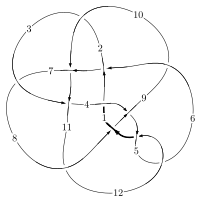
\includegraphics[width=112pt]{../../../GIT/diagram.site/Diagrams/png/1994_12a_1193.png}\\
\ \ \ A knot diagram\footnotemark}&
\allowdisplaybreaks
\textbf{Linearized knot diagam} \\
\cline{2-2}
 &
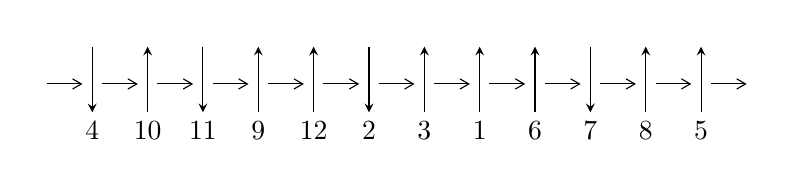
\begin{tikzpicture}[x=20pt, y=17pt]
	% nodes
	\node (C0) at (0, 0) {};
	\node (C1) at (1, 0) {};
	\node (C1U) at (1, +1) {};
	\node (C1D) at (1, -1) {4};

	\node (C2) at (2, 0) {};
	\node (C2U) at (2, +1) {};
	\node (C2D) at (2, -1) {10};

	\node (C3) at (3, 0) {};
	\node (C3U) at (3, +1) {};
	\node (C3D) at (3, -1) {11};

	\node (C4) at (4, 0) {};
	\node (C4U) at (4, +1) {};
	\node (C4D) at (4, -1) {9};

	\node (C5) at (5, 0) {};
	\node (C5U) at (5, +1) {};
	\node (C5D) at (5, -1) {12};

	\node (C6) at (6, 0) {};
	\node (C6U) at (6, +1) {};
	\node (C6D) at (6, -1) {2};

	\node (C7) at (7, 0) {};
	\node (C7U) at (7, +1) {};
	\node (C7D) at (7, -1) {3};

	\node (C8) at (8, 0) {};
	\node (C8U) at (8, +1) {};
	\node (C8D) at (8, -1) {1};

	\node (C9) at (9, 0) {};
	\node (C9U) at (9, +1) {};
	\node (C9D) at (9, -1) {6};

	\node (C10) at (10, 0) {};
	\node (C10U) at (10, +1) {};
	\node (C10D) at (10, -1) {7};

	\node (C11) at (11, 0) {};
	\node (C11U) at (11, +1) {};
	\node (C11D) at (11, -1) {8};

	\node (C12) at (12, 0) {};
	\node (C12U) at (12, +1) {};
	\node (C12D) at (12, -1) {5};
	\node (C13) at (13, 0) {};

	% arrows
	\draw[->,>={angle 60}]
	(C0) edge (C1) (C1) edge (C2) (C2) edge (C3) (C3) edge (C4) (C4) edge (C5) (C5) edge (C6) (C6) edge (C7) (C7) edge (C8) (C8) edge (C9) (C9) edge (C10) (C10) edge (C11) (C11) edge (C12) (C12) edge (C13) ;	\draw[->,>=stealth]
	(C1U) edge (C1D) (C2D) edge (C2U) (C3U) edge (C3D) (C4D) edge (C4U) (C5D) edge (C5U) (C6U) edge (C6D) (C7D) edge (C7U) (C8D) edge (C8U) (C9D) edge (C9U) (C10U) edge (C10D) (C11D) edge (C11U) (C12D) edge (C12U) ;
	\end{tikzpicture} \\
\hhline{~~} \\& 
\textbf{Solving Sequence} \\ \cline{2-2} 
 &
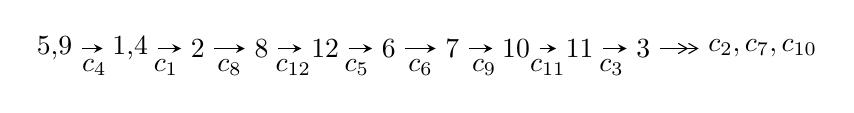
\begin{tikzpicture}[x=23pt, y=7pt]
	% node
	\node (A0) at (-1/8, 0) {5,9};
	\node (A1) at (17/16, 0) {1,4};
	\node (A2) at (17/8, 0) {2};
	\node (A3) at (25/8, 0) {8};
	\node (A4) at (33/8, 0) {12};
	\node (A5) at (41/8, 0) {6};
	\node (A6) at (49/8, 0) {7};
	\node (A7) at (57/8, 0) {10};
	\node (A8) at (65/8, 0) {11};
	\node (A9) at (73/8, 0) {3};
	\node (C1) at (1/2, -1) {$c_{4}$};
	\node (C2) at (13/8, -1) {$c_{1}$};
	\node (C3) at (21/8, -1) {$c_{8}$};
	\node (C4) at (29/8, -1) {$c_{12}$};
	\node (C5) at (37/8, -1) {$c_{5}$};
	\node (C6) at (45/8, -1) {$c_{6}$};
	\node (C7) at (53/8, -1) {$c_{9}$};
	\node (C8) at (61/8, -1) {$c_{11}$};
	\node (C9) at (69/8, -1) {$c_{3}$};
	\node (A10) at (11, 0) {$c_{2},c_{7},c_{10}$};

	% edge
	\draw[->,>=stealth]	
	(A0) edge (A1) (A1) edge (A2) (A2) edge (A3) (A3) edge (A4) (A4) edge (A5) (A5) edge (A6) (A6) edge (A7) (A7) edge (A8) (A8) edge (A9) ;
	\draw[->>,>={angle 60}]	
	(A9) edge (A10);
\end{tikzpicture} \\ 

\end{tabular} \\

\footnotetext{
The image of knot diagram is generated by the software ``\textbf{Draw programme}" developed by Andrew Bartholomew(\url{http://www.layer8.co.uk/maths/draw/index.htm\#Running-draw}), where we modified some parts for our purpose(\url{https://github.com/CATsTAILs/LinksPainter}).
}\phantom \\ \newline 
\centering \textbf{Ideals for irreducible components\footnotemark of $X_{\text{par}}$} 
 
\begin{align*}
I^u_{1}&=\langle 
1.94312\times10^{80} u^{49}-2.48619\times10^{79} u^{48}+\cdots+7.87680\times10^{79} b+1.28241\times10^{80},\;a-1,\\
\phantom{I^u_{1}}&\phantom{= \langle  }u^{50}+5 u^{48}+\cdots+5 u+1\rangle \\
I^u_{2}&=\langle 
1.63014\times10^{1735} u^{155}-9.72983\times10^{1735} u^{154}+\cdots+1.03065\times10^{1738} b+8.61106\times10^{1738},\\
\phantom{I^u_{2}}&\phantom{= \langle  }1.64322\times10^{1736} u^{155}-2.98949\times10^{1735} u^{154}+\cdots+4.74098\times10^{1739} a+1.16259\times10^{1741},\\
\phantom{I^u_{2}}&\phantom{= \langle  }u^{156}-6 u^{155}+\cdots+6790 u+1288\rangle \\
I^u_{3}&=\langle 
-5.51879\times10^{28} u^{32}+2.59045\times10^{28} u^{31}+\cdots+5.79727\times10^{28} b-5.00823\times10^{27},\;a+1,\\
\phantom{I^u_{3}}&\phantom{= \langle  }u^{33}+5 u^{31}+\cdots+4 u+1\rangle \\
I^u_{4}&=\langle 
-484122 u^{11}-2829135 u^{10}+\cdots+24262754 b+7309133,\\
\phantom{I^u_{4}}&\phantom{= \langle  }19820339 u^{11}+138389241 u^{10}+\cdots+48525508 a-191613318,\\
\phantom{I^u_{4}}&\phantom{= \langle  }u^{12}+7 u^{11}+16 u^{10}+12 u^9+9 u^8+29 u^7+43 u^6+6 u^5+3 u^4+38 u^3+7 u^2-6 u+8\rangle \\
\\
\end{align*}
\raggedright * 4 irreducible components of $\dim_{\mathbb{C}}=0$, with total 251 representations.\\
\footnotetext{All coefficients of polynomials are rational numbers. But the coefficients are sometimes approximated in decimal forms when there is not enough margin.}
\newpage
\renewcommand{\arraystretch}{1}
\centering \section*{I. $I^u_{1}= \langle 1.94\times10^{80} u^{49}-2.49\times10^{79} u^{48}+\cdots+7.88\times10^{79} b+1.28\times10^{80},\;a-1,\;u^{50}+5 u^{48}+\cdots+5 u+1 \rangle$}
\flushleft \textbf{(i) Arc colorings}\\
\begin{tabular}{m{7pt} m{180pt} m{7pt} m{180pt} }
\flushright $a_{5}=$&$\begin{pmatrix}1\\0\end{pmatrix}$ \\
\flushright $a_{9}=$&$\begin{pmatrix}0\\u\end{pmatrix}$ \\
\flushright $a_{1}=$&$\begin{pmatrix}1\\-2.46689 u^{49}+0.315634 u^{48}+\cdots-30.2403 u-1.62809\end{pmatrix}$ \\
\flushright $a_{4}=$&$\begin{pmatrix}1\\u^2\end{pmatrix}$ \\
\flushright $a_{2}=$&$\begin{pmatrix}2.46689 u^{49}-0.315634 u^{48}+\cdots+30.2403 u+2.62809\\-2.59720 u^{49}+0.343485 u^{48}+\cdots-31.1290 u-1.31245\end{pmatrix}$ \\
\flushright $a_{8}=$&$\begin{pmatrix}- u\\-0.315634 u^{49}-0.130315 u^{48}+\cdots-9.70634 u-2.46689\end{pmatrix}$ \\
\flushright $a_{12}=$&$\begin{pmatrix}2.46689 u^{49}-0.315634 u^{48}+\cdots+30.2403 u+2.62809\\-2.46689 u^{49}+0.315634 u^{48}+\cdots-30.2403 u-1.62809\end{pmatrix}$ \\
\flushright $a_{6}=$&$\begin{pmatrix}0.723740 u^{49}-0.524718 u^{48}+\cdots+6.95916 u-5.96362\\1.74315 u^{49}+0.209084 u^{48}+\cdots+23.2812 u+8.59171\end{pmatrix}$ \\
\flushright $a_{7}=$&$\begin{pmatrix}1.29977 u^{49}+0.0121696 u^{48}+\cdots+13.6811 u-0.964916\\-0.327667 u^{49}-0.224139 u^{48}+\cdots-5.88790 u+1.64958\end{pmatrix}$ \\
\flushright $a_{10}=$&$\begin{pmatrix}1.17574 u^{49}+0.670154 u^{48}+\cdots+56.3848 u+11.9751\\-1.61868 u^{49}+0.605612 u^{48}+\cdots-38.8939 u-4.19712\end{pmatrix}$ \\
\flushright $a_{11}=$&$\begin{pmatrix}2.16799 u^{49}-0.221391 u^{48}+\cdots+28.3405 u+2.10337\\-1.19112 u^{49}+0.0824317 u^{48}+\cdots-20.2477 u-1.18515\end{pmatrix}$ \\
\flushright $a_{3}=$&$\begin{pmatrix}-1.17145 u^{49}-0.615972 u^{48}+\cdots-14.7992 u-4.90764\\1.33864 u^{49}+0.700909 u^{48}+\cdots+28.4451 u+6.40340\end{pmatrix}$\\&\end{tabular}
\flushleft \textbf{(ii) Obstruction class $= -1$}\\~\\
\flushleft \textbf{(iii) Cusp Shapes $= 16.2604 u^{49}-4.35079 u^{48}+\cdots+259.730 u+13.6919$}\\~\\
\newpage\renewcommand{\arraystretch}{1}
\flushleft \textbf{(iv) u-Polynomials at the component}\newline \\
\begin{tabular}{m{50pt}|m{274pt}}
Crossings & \hspace{64pt}u-Polynomials at each crossing \\
\hline $$\begin{aligned}c_{1}\end{aligned}$$&$\begin{aligned}
&u^{50}-37 u^{49}+\cdots-1343488 u+65536
\end{aligned}$\\
\hline $$\begin{aligned}c_{2},c_{7}\end{aligned}$$&$\begin{aligned}
&u^{50}+u^{49}+\cdots+u+1
\end{aligned}$\\
\hline $$\begin{aligned}c_{3},c_{6}\end{aligned}$$&$\begin{aligned}
&u^{50}+u^{49}+\cdots+u+1
\end{aligned}$\\
\hline $$\begin{aligned}c_{4},c_{8}\end{aligned}$$&$\begin{aligned}
&u^{50}+5 u^{48}+\cdots+5 u+1
\end{aligned}$\\
\hline $$\begin{aligned}c_{5},c_{12}\end{aligned}$$&$\begin{aligned}
&u^{50}-27 u^{49}+\cdots-45312 u+2560
\end{aligned}$\\
\hline $$\begin{aligned}c_{9},c_{11}\end{aligned}$$&$\begin{aligned}
&u^{50}+2 u^{49}+\cdots-284 u+148
\end{aligned}$\\
\hline $$\begin{aligned}c_{10}\end{aligned}$$&$\begin{aligned}
&u^{50}+33 u^{49}+\cdots+3584 u+256
\end{aligned}$\\
\hline
\end{tabular}\\~\\
\newpage\renewcommand{\arraystretch}{1}
\flushleft \textbf{(v) Riley Polynomials at the component}\newline \\
\begin{tabular}{m{50pt}|m{274pt}}
Crossings & \hspace{64pt}Riley Polynomials at each crossing \\
\hline $$\begin{aligned}c_{1}\end{aligned}$$&$\begin{aligned}
&y^{50}+15 y^{49}+\cdots+68719476736 y+4294967296
\end{aligned}$\\
\hline $$\begin{aligned}c_{2},c_{7}\end{aligned}$$&$\begin{aligned}
&y^{50}-23 y^{49}+\cdots-51 y+1
\end{aligned}$\\
\hline $$\begin{aligned}c_{3},c_{6}\end{aligned}$$&$\begin{aligned}
&y^{50}+5 y^{49}+\cdots+29 y+1
\end{aligned}$\\
\hline $$\begin{aligned}c_{4},c_{8}\end{aligned}$$&$\begin{aligned}
&y^{50}+10 y^{49}+\cdots+37 y+1
\end{aligned}$\\
\hline $$\begin{aligned}c_{5},c_{12}\end{aligned}$$&$\begin{aligned}
&y^{50}+35 y^{49}+\cdots+254345216 y+6553600
\end{aligned}$\\
\hline $$\begin{aligned}c_{9},c_{11}\end{aligned}$$&$\begin{aligned}
&y^{50}-12 y^{49}+\cdots-46320 y+21904
\end{aligned}$\\
\hline $$\begin{aligned}c_{10}\end{aligned}$$&$\begin{aligned}
&y^{50}+7 y^{49}+\cdots+1769472 y+65536
\end{aligned}$\\
\hline
\end{tabular}\\~\\
\newpage\flushleft \textbf{(vi) Complex Volumes and Cusp Shapes}
$$\begin{array}{c|c|c}  
\text{Solutions to }I^u_{1}& \I (\text{vol} + \sqrt{-1}CS) & \text{Cusp shape}\\
 \hline 
\begin{aligned}
u &= -0.643464 + 0.769213 I \\
a &= \phantom{-}1.00000\phantom{ +0.000000I} \\
b &= \phantom{-}1.166190 + 0.558776 I\end{aligned}
 & \phantom{-}4.36390 - 1.77312 I & \phantom{-}8.40093 + 4.75657 I \\ \hline\begin{aligned}
u &= -0.643464 - 0.769213 I \\
a &= \phantom{-}1.00000\phantom{ +0.000000I} \\
b &= \phantom{-}1.166190 - 0.558776 I\end{aligned}
 & \phantom{-}4.36390 + 1.77312 I & \phantom{-}8.40093 - 4.75657 I \\ \hline\begin{aligned}
u &= -0.209680 + 0.984180 I \\
a &= \phantom{-}1.00000\phantom{ +0.000000I} \\
b &= \phantom{-}0.982677 - 0.823149 I\end{aligned}
 & -0.65225 + 5.66298 I & \phantom{-}1.39055 - 3.29167 I \\ \hline\begin{aligned}
u &= -0.209680 - 0.984180 I \\
a &= \phantom{-}1.00000\phantom{ +0.000000I} \\
b &= \phantom{-}0.982677 + 0.823149 I\end{aligned}
 & -0.65225 - 5.66298 I & \phantom{-}1.39055 + 3.29167 I \\ \hline\begin{aligned}
u &= \phantom{-}0.111854 + 0.935193 I \\
a &= \phantom{-}1.00000\phantom{ +0.000000I} \\
b &= \phantom{-}0.014940 - 0.254880 I\end{aligned}
 & -2.13721 + 4.98350 I & -0.46686 - 6.95288 I \\ \hline\begin{aligned}
u &= \phantom{-}0.111854 - 0.935193 I \\
a &= \phantom{-}1.00000\phantom{ +0.000000I} \\
b &= \phantom{-}0.014940 + 0.254880 I\end{aligned}
 & -2.13721 - 4.98350 I & -0.46686 + 6.95288 I \\ \hline\begin{aligned}
u &= \phantom{-}0.454709 + 0.811898 I \\
a &= \phantom{-}1.00000\phantom{ +0.000000I} \\
b &= \phantom{-}0.73450 + 1.36481 I\end{aligned}
 & \phantom{-}0.29883 + 6.52796 I & \phantom{-}4.59641 - 9.04204 I \\ \hline\begin{aligned}
u &= \phantom{-}0.454709 - 0.811898 I \\
a &= \phantom{-}1.00000\phantom{ +0.000000I} \\
b &= \phantom{-}0.73450 - 1.36481 I\end{aligned}
 & \phantom{-}0.29883 - 6.52796 I & \phantom{-}4.59641 + 9.04204 I \\ \hline\begin{aligned}
u &= -0.792910 + 0.423437 I \\
a &= \phantom{-}1.00000\phantom{ +0.000000I} \\
b &= \phantom{-}1.176340 + 0.218285 I\end{aligned}
 & \phantom{-}5.47703 - 0.93007 I & \phantom{-}13.31306 + 3.09237 I \\ \hline\begin{aligned}
u &= -0.792910 - 0.423437 I \\
a &= \phantom{-}1.00000\phantom{ +0.000000I} \\
b &= \phantom{-}1.176340 - 0.218285 I\end{aligned}
 & \phantom{-}5.47703 + 0.93007 I & \phantom{-}13.31306 - 3.09237 I\\
 \hline 
 \end{array}$$\newpage$$\begin{array}{c|c|c}  
\text{Solutions to }I^u_{1}& \I (\text{vol} + \sqrt{-1}CS) & \text{Cusp shape}\\
 \hline 
\begin{aligned}
u &= -0.892105 + 0.668186 I \\
a &= \phantom{-}1.00000\phantom{ +0.000000I} \\
b &= \phantom{-}1.277600 + 0.060374 I\end{aligned}
 & \phantom{-}6.15364 - 7.17141 I & \phantom{-}12.2491 + 7.9503 I \\ \hline\begin{aligned}
u &= -0.892105 - 0.668186 I \\
a &= \phantom{-}1.00000\phantom{ +0.000000I} \\
b &= \phantom{-}1.277600 - 0.060374 I\end{aligned}
 & \phantom{-}6.15364 + 7.17141 I & \phantom{-}12.2491 - 7.9503 I \\ \hline\begin{aligned}
u &= -0.726926 + 0.378293 I \\
a &= \phantom{-}1.00000\phantom{ +0.000000I} \\
b &= \phantom{-}0.262626 - 1.136960 I\end{aligned}
 & -1.59993 - 2.70489 I & \phantom{-}3.40729 + 2.86854 I \\ \hline\begin{aligned}
u &= -0.726926 - 0.378293 I \\
a &= \phantom{-}1.00000\phantom{ +0.000000I} \\
b &= \phantom{-}0.262626 + 1.136960 I\end{aligned}
 & -1.59993 + 2.70489 I & \phantom{-}3.40729 - 2.86854 I \\ \hline\begin{aligned}
u &= \phantom{-}0.727284 + 0.360560 I \\
a &= \phantom{-}1.00000\phantom{ +0.000000I} \\
b &= \phantom{-}0.620921 + 0.171349 I\end{aligned}
 & \phantom{-}1.246370 + 0.482488 I & \phantom{-}7.31465 - 2.33574 I \\ \hline\begin{aligned}
u &= \phantom{-}0.727284 - 0.360560 I \\
a &= \phantom{-}1.00000\phantom{ +0.000000I} \\
b &= \phantom{-}0.620921 - 0.171349 I\end{aligned}
 & \phantom{-}1.246370 - 0.482488 I & \phantom{-}7.31465 + 2.33574 I \\ \hline\begin{aligned}
u &= \phantom{-}0.909966 + 0.776093 I \\
a &= \phantom{-}1.00000\phantom{ +0.000000I} \\
b &= \phantom{-}1.241250 - 0.156499 I\end{aligned}
 & \phantom{-}4.5544 + 15.8113 I & \phantom{-0.000000 } 0 \\ \hline\begin{aligned}
u &= \phantom{-}0.909966 - 0.776093 I \\
a &= \phantom{-}1.00000\phantom{ +0.000000I} \\
b &= \phantom{-}1.241250 + 0.156499 I\end{aligned}
 & \phantom{-}4.5544 - 15.8113 I & \phantom{-0.000000 } 0 \\ \hline\begin{aligned}
u &= -0.324125 + 1.157810 I \\
a &= \phantom{-}1.00000\phantom{ +0.000000I} \\
b &= \phantom{-}0.79105 - 1.25368 I\end{aligned}
 & -2.24034 - 12.75630 I & \phantom{-0.000000 } 0 \\ \hline\begin{aligned}
u &= -0.324125 - 1.157810 I \\
a &= \phantom{-}1.00000\phantom{ +0.000000I} \\
b &= \phantom{-}0.79105 + 1.25368 I\end{aligned}
 & -2.24034 + 12.75630 I & \phantom{-0.000000 } 0\\
 \hline 
 \end{array}$$\newpage$$\begin{array}{c|c|c}  
\text{Solutions to }I^u_{1}& \I (\text{vol} + \sqrt{-1}CS) & \text{Cusp shape}\\
 \hline 
\begin{aligned}
u &= \phantom{-}0.952387 + 0.735226 I \\
a &= \phantom{-}1.00000\phantom{ +0.000000I} \\
b &= \phantom{-}0.892872 - 0.485258 I\end{aligned}
 & \phantom{-}5.37270 - 1.91715 I & \phantom{-0.000000 } 0 \\ \hline\begin{aligned}
u &= \phantom{-}0.952387 - 0.735226 I \\
a &= \phantom{-}1.00000\phantom{ +0.000000I} \\
b &= \phantom{-}0.892872 + 0.485258 I\end{aligned}
 & \phantom{-}5.37270 + 1.91715 I & \phantom{-0.000000 } 0 \\ \hline\begin{aligned}
u &= -0.338470 + 0.671302 I \\
a &= \phantom{-}1.00000\phantom{ +0.000000I} \\
b &= -0.063362 - 1.273950 I\end{aligned}
 & -4.46772 - 0.64019 I & -2.99722 + 2.10098 I \\ \hline\begin{aligned}
u &= -0.338470 - 0.671302 I \\
a &= \phantom{-}1.00000\phantom{ +0.000000I} \\
b &= -0.063362 + 1.273950 I\end{aligned}
 & -4.46772 + 0.64019 I & -2.99722 - 2.10098 I \\ \hline\begin{aligned}
u &= \phantom{-}0.394993 + 0.596716 I \\
a &= \phantom{-}1.00000\phantom{ +0.000000I} \\
b &= \phantom{-}0.933205 + 0.993015 I\end{aligned}
 & \phantom{-}2.14090 + 1.30641 I & \phantom{-}7.07669 - 7.35081 I \\ \hline\begin{aligned}
u &= \phantom{-}0.394993 - 0.596716 I \\
a &= \phantom{-}1.00000\phantom{ +0.000000I} \\
b &= \phantom{-}0.933205 - 0.993015 I\end{aligned}
 & \phantom{-}2.14090 - 1.30641 I & \phantom{-}7.07669 + 7.35081 I \\ \hline\begin{aligned}
u &= \phantom{-}1.026820 + 0.792152 I \\
a &= \phantom{-}1.00000\phantom{ +0.000000I} \\
b &= -0.027990 + 0.832206 I\end{aligned}
 & \phantom{-}0.92663 - 2.16938 I & \phantom{-0.000000 } 0 \\ \hline\begin{aligned}
u &= \phantom{-}1.026820 - 0.792152 I \\
a &= \phantom{-}1.00000\phantom{ +0.000000I} \\
b &= -0.027990 - 0.832206 I\end{aligned}
 & \phantom{-}0.92663 + 2.16938 I & \phantom{-0.000000 } 0 \\ \hline\begin{aligned}
u &= \phantom{-}0.641768 + 1.157350 I \\
a &= \phantom{-}1.00000\phantom{ +0.000000I} \\
b &= \phantom{-}0.186450 + 1.239270 I\end{aligned}
 & -6.86303 - 3.75834 I & \phantom{-0.000000 } 0 \\ \hline\begin{aligned}
u &= \phantom{-}0.641768 - 1.157350 I \\
a &= \phantom{-}1.00000\phantom{ +0.000000I} \\
b &= \phantom{-}0.186450 - 1.239270 I\end{aligned}
 & -6.86303 + 3.75834 I & \phantom{-0.000000 } 0\\
 \hline 
 \end{array}$$\newpage$$\begin{array}{c|c|c}  
\text{Solutions to }I^u_{1}& \I (\text{vol} + \sqrt{-1}CS) & \text{Cusp shape}\\
 \hline 
\begin{aligned}
u &= -0.901999 + 1.045100 I \\
a &= \phantom{-}1.00000\phantom{ +0.000000I} \\
b &= \phantom{-}0.293959 - 1.351620 I\end{aligned}
 & -3.65978 - 3.90185 I & \phantom{-0.000000 } 0 \\ \hline\begin{aligned}
u &= -0.901999 - 1.045100 I \\
a &= \phantom{-}1.00000\phantom{ +0.000000I} \\
b &= \phantom{-}0.293959 + 1.351620 I\end{aligned}
 & -3.65978 + 3.90185 I & \phantom{-0.000000 } 0 \\ \hline\begin{aligned}
u &= \phantom{-}1.000200 + 0.965591 I \\
a &= \phantom{-}1.00000\phantom{ +0.000000I} \\
b &= \phantom{-}0.62065 + 1.29063 I\end{aligned}
 & \phantom{-}2.08227 + 7.18268 I & \phantom{-0.000000 } 0 \\ \hline\begin{aligned}
u &= \phantom{-}1.000200 - 0.965591 I \\
a &= \phantom{-}1.00000\phantom{ +0.000000I} \\
b &= \phantom{-}0.62065 - 1.29063 I\end{aligned}
 & \phantom{-}2.08227 - 7.18268 I & \phantom{-0.000000 } 0 \\ \hline\begin{aligned}
u &= -0.84268 + 1.17438 I \\
a &= \phantom{-}1.00000\phantom{ +0.000000I} \\
b &= \phantom{-}0.057255 - 1.186230 I\end{aligned}
 & -5.01603 - 5.20693 I & \phantom{-0.000000 } 0 \\ \hline\begin{aligned}
u &= -0.84268 - 1.17438 I \\
a &= \phantom{-}1.00000\phantom{ +0.000000I} \\
b &= \phantom{-}0.057255 + 1.186230 I\end{aligned}
 & -5.01603 + 5.20693 I & \phantom{-0.000000 } 0 \\ \hline\begin{aligned}
u &= \phantom{-}0.94208 + 1.19268 I \\
a &= \phantom{-}1.00000\phantom{ +0.000000I} \\
b &= \phantom{-}0.694329 + 1.176010 I\end{aligned}
 & \phantom{-}2.17532 + 8.34585 I & \phantom{-0.000000 } 0 \\ \hline\begin{aligned}
u &= \phantom{-}0.94208 - 1.19268 I \\
a &= \phantom{-}1.00000\phantom{ +0.000000I} \\
b &= \phantom{-}0.694329 - 1.176010 I\end{aligned}
 & \phantom{-}2.17532 - 8.34585 I & \phantom{-0.000000 } 0 \\ \hline\begin{aligned}
u &= -0.195613 + 0.426357 I \\
a &= \phantom{-}1.00000\phantom{ +0.000000I} \\
b &= -0.216338 + 0.544332 I\end{aligned}
 & \phantom{-}0.50466 + 1.79559 I & \phantom{-}3.46378 - 3.10051 I \\ \hline\begin{aligned}
u &= -0.195613 - 0.426357 I \\
a &= \phantom{-}1.00000\phantom{ +0.000000I} \\
b &= -0.216338 - 0.544332 I\end{aligned}
 & \phantom{-}0.50466 - 1.79559 I & \phantom{-}3.46378 + 3.10051 I\\
 \hline 
 \end{array}$$\newpage$$\begin{array}{c|c|c}  
\text{Solutions to }I^u_{1}& \I (\text{vol} + \sqrt{-1}CS) & \text{Cusp shape}\\
 \hline 
\begin{aligned}
u &= -0.015924 + 0.425046 I \\
a &= \phantom{-}1.00000\phantom{ +0.000000I} \\
b &= \phantom{-}0.06103 + 1.82231 I\end{aligned}
 & -2.19516 - 9.28833 I & -7.03273 + 5.74266 I \\ \hline\begin{aligned}
u &= -0.015924 - 0.425046 I \\
a &= \phantom{-}1.00000\phantom{ +0.000000I} \\
b &= \phantom{-}0.06103 - 1.82231 I\end{aligned}
 & -2.19516 + 9.28833 I & -7.03273 - 5.74266 I \\ \hline\begin{aligned}
u &= \phantom{-}1.07924 + 1.18155 I \\
a &= \phantom{-}1.00000\phantom{ +0.000000I} \\
b &= \phantom{-}0.62297 + 1.37503 I\end{aligned}
 & \phantom{-}2.04993 + 13.72580 I & \phantom{-0.000000 } 0 \\ \hline\begin{aligned}
u &= \phantom{-}1.07924 - 1.18155 I \\
a &= \phantom{-}1.00000\phantom{ +0.000000I} \\
b &= \phantom{-}0.62297 - 1.37503 I\end{aligned}
 & \phantom{-}2.04993 - 13.72580 I & \phantom{-0.000000 } 0 \\ \hline\begin{aligned}
u &= -1.12239 + 1.17529 I \\
a &= \phantom{-}1.00000\phantom{ +0.000000I} \\
b &= \phantom{-}0.584184 - 1.132490 I\end{aligned}
 & \phantom{-}3.25548 - 3.52615 I & \phantom{-0.000000 } 0 \\ \hline\begin{aligned}
u &= -1.12239 - 1.17529 I \\
a &= \phantom{-}1.00000\phantom{ +0.000000I} \\
b &= \phantom{-}0.584184 + 1.132490 I\end{aligned}
 & \phantom{-}3.25548 + 3.52615 I & \phantom{-0.000000 } 0 \\ \hline\begin{aligned}
u &= -1.10707 + 1.25249 I \\
a &= \phantom{-}1.00000\phantom{ +0.000000I} \\
b &= \phantom{-}0.63231 - 1.34103 I\end{aligned}
 & \phantom{-}0.8116 - 22.3107 I & \phantom{-0.000000 } 0 \\ \hline\begin{aligned}
u &= -1.10707 - 1.25249 I \\
a &= \phantom{-}1.00000\phantom{ +0.000000I} \\
b &= \phantom{-}0.63231 + 1.34103 I\end{aligned}
 & \phantom{-}0.8116 + 22.3107 I & \phantom{-0.000000 } 0 \\ \hline\begin{aligned}
u &= -0.127947 + 0.260665 I \\
a &= \phantom{-}1.00000\phantom{ +0.000000I} \\
b &= -0.03961 - 2.00425 I\end{aligned}
 & -0.245250 - 0.513655 I & \phantom{-}1.5494 + 26.0988 I \\ \hline\begin{aligned}
u &= -0.127947 - 0.260665 I \\
a &= \phantom{-}1.00000\phantom{ +0.000000I} \\
b &= -0.03961 + 2.00425 I\end{aligned}
 & -0.245250 + 0.513655 I & \phantom{-}1.5494 - 26.0988 I\\
 \hline 
 \end{array}$$\newpage\newpage\renewcommand{\arraystretch}{1}
\centering \section*{II. $I^u_{2}= \langle 1.63\times10^{1735} u^{155}-9.73\times10^{1735} u^{154}+\cdots+1.03\times10^{1738} b+8.61\times10^{1738},\;1.64\times10^{1736} u^{155}-2.99\times10^{1735} u^{154}+\cdots+4.74\times10^{1739} a+1.16\times10^{1741},\;u^{156}-6 u^{155}+\cdots+6790 u+1288 \rangle$}
\flushleft \textbf{(i) Arc colorings}\\
\begin{tabular}{m{7pt} m{180pt} m{7pt} m{180pt} }
\flushright $a_{5}=$&$\begin{pmatrix}1\\0\end{pmatrix}$ \\
\flushright $a_{9}=$&$\begin{pmatrix}0\\u\end{pmatrix}$ \\
\flushright $a_{1}=$&$\begin{pmatrix}-0.000346599 u^{155}+0.0000630564 u^{154}+\cdots-49.7051 u-24.5222\\-0.00158166 u^{155}+0.00944050 u^{154}+\cdots-37.3726 u-8.35500\end{pmatrix}$ \\
\flushright $a_{4}=$&$\begin{pmatrix}1\\u^2\end{pmatrix}$ \\
\flushright $a_{2}=$&$\begin{pmatrix}0.00204685 u^{155}-0.0143357 u^{154}+\cdots+1.80622 u-13.5699\\-0.00179839 u^{155}+0.0108199 u^{154}+\cdots-40.1971 u-8.30601\end{pmatrix}$ \\
\flushright $a_{8}=$&$\begin{pmatrix}0.0101130 u^{155}-0.0591571 u^{154}+\cdots+470.090 u+66.8018\\-0.00337653 u^{155}+0.0205497 u^{154}+\cdots-77.3509 u-11.1044\end{pmatrix}$ \\
\flushright $a_{12}=$&$\begin{pmatrix}0.00123506 u^{155}-0.00937744 u^{154}+\cdots-12.3325 u-16.1672\\-0.00158166 u^{155}+0.00944050 u^{154}+\cdots-37.3726 u-8.35500\end{pmatrix}$ \\
\flushright $a_{6}=$&$\begin{pmatrix}0.00847347 u^{155}-0.0528439 u^{154}+\cdots+95.8064 u-2.97935\\0.000148000 u^{155}-0.00226143 u^{154}+\cdots-32.9533 u-15.8318\end{pmatrix}$ \\
\flushright $a_{7}=$&$\begin{pmatrix}-0.000693818 u^{155}+0.00122309 u^{154}+\cdots-91.8035 u-44.3276\\0.00200736 u^{155}-0.0119787 u^{154}+\cdots+42.5562 u+9.89170\end{pmatrix}$ \\
\flushright $a_{10}=$&$\begin{pmatrix}0.0195170 u^{155}-0.119912 u^{154}+\cdots+571.122 u+56.6772\\-0.00440003 u^{155}+0.0264988 u^{154}+\cdots-105.520 u-18.8433\end{pmatrix}$ \\
\flushright $a_{11}=$&$\begin{pmatrix}0.00770984 u^{155}-0.0439725 u^{154}+\cdots+433.571 u+68.3438\\-0.000999740 u^{155}+0.00558199 u^{154}+\cdots-45.2645 u-10.1410\end{pmatrix}$ \\
\flushright $a_{3}=$&$\begin{pmatrix}0.0137587 u^{155}-0.0844136 u^{154}+\cdots-63.9818 u-42.9558\\-0.00167335 u^{155}+0.0107474 u^{154}+\cdots-17.9859 u+5.76366\end{pmatrix}$\\&\end{tabular}
\flushleft \textbf{(ii) Obstruction class $= -1$}\\~\\
\flushleft \textbf{(iii) Cusp Shapes $= -0.0125289 u^{155}+0.0675500 u^{154}+\cdots-444.155 u-151.722$}\\~\\
\newpage\renewcommand{\arraystretch}{1}
\flushleft \textbf{(iv) u-Polynomials at the component}\newline \\
\begin{tabular}{m{50pt}|m{274pt}}
Crossings & \hspace{64pt}u-Polynomials at each crossing \\
\hline $$\begin{aligned}c_{1}\end{aligned}$$&$\begin{aligned}
&4(2 u^{78}+47 u^{77}+\cdots+1391 u+71)^{2}
\end{aligned}$\\
\hline $$\begin{aligned}c_{2},c_{7}\end{aligned}$$&$\begin{aligned}
&u^{156}-2 u^{155}+\cdots-932767 u-85726
\end{aligned}$\\
\hline $$\begin{aligned}c_{3},c_{6}\end{aligned}$$&$\begin{aligned}
&2(2 u^{156}-11 u^{155}+\cdots-10689 u+882)
\end{aligned}$\\
\hline $$\begin{aligned}c_{4},c_{8}\end{aligned}$$&$\begin{aligned}
&u^{156}-6 u^{155}+\cdots+6790 u+1288
\end{aligned}$\\
\hline $$\begin{aligned}c_{5},c_{12}\end{aligned}$$&$\begin{aligned}
&4(2 u^{78}+29 u^{77}+\cdots+2 u-1)^{2}
\end{aligned}$\\
\hline $$\begin{aligned}c_{9},c_{11}\end{aligned}$$&$\begin{aligned}
&2(2 u^{156}+9 u^{155}+\cdots-1.96661\times10^{11} u+9.82273\times10^{9})
\end{aligned}$\\
\hline $$\begin{aligned}c_{10}\end{aligned}$$&$\begin{aligned}
&4(2 u^{78}-33 u^{77}+\cdots-13 u+1)^{2}
\end{aligned}$\\
\hline
\end{tabular}\\~\\
\newpage\renewcommand{\arraystretch}{1}
\flushleft \textbf{(v) Riley Polynomials at the component}\newline \\
\begin{tabular}{m{50pt}|m{274pt}}
Crossings & \hspace{64pt}Riley Polynomials at each crossing \\
\hline $$\begin{aligned}c_{1}\end{aligned}$$&$\begin{aligned}
&16(4 y^{78}+67 y^{77}+\cdots-256583 y+5041)^{2}
\end{aligned}$\\
\hline $$\begin{aligned}c_{2},c_{7}\end{aligned}$$&$\begin{aligned}
&y^{156}+6 y^{155}+\cdots-628310042425 y+7348947076
\end{aligned}$\\
\hline $$\begin{aligned}c_{3},c_{6}\end{aligned}$$&$\begin{aligned}
&4(4 y^{156}-y^{155}+\cdots-5.42417\times10^{7} y+777924)
\end{aligned}$\\
\hline $$\begin{aligned}c_{4},c_{8}\end{aligned}$$&$\begin{aligned}
&y^{156}-6 y^{155}+\cdots+68705644 y+1658944
\end{aligned}$\\
\hline $$\begin{aligned}c_{5},c_{12}\end{aligned}$$&$\begin{aligned}
&16(4 y^{78}+191 y^{77}+\cdots+2 y+1)^{2}
\end{aligned}$\\
\hline $$\begin{aligned}c_{9},c_{11}\end{aligned}$$&$\begin{aligned}
&4(4 y^{156}-225 y^{155}+\cdots-3.03964\times10^{22} y+9.64861\times10^{19})
\end{aligned}$\\
\hline $$\begin{aligned}c_{10}\end{aligned}$$&$\begin{aligned}
&16(4 y^{78}-37 y^{77}+\cdots-57 y+1)^{2}
\end{aligned}$\\
\hline
\end{tabular}\\~\\
\newpage\flushleft \textbf{(vi) Complex Volumes and Cusp Shapes}
$$\begin{array}{c|c|c}  
\text{Solutions to }I^u_{2}& \I (\text{vol} + \sqrt{-1}CS) & \text{Cusp shape}\\
 \hline 
\begin{aligned}
u &= \phantom{-}0.479961 + 0.895187 I \\
a &= -1.50431 + 0.97086 I \\
b &= -0.315677 - 1.273790 I\end{aligned}
 & -2.85447 + 1.56373 I & \phantom{-0.000000 } 0 \\ \hline\begin{aligned}
u &= \phantom{-}0.479961 - 0.895187 I \\
a &= -1.50431 - 0.97086 I \\
b &= -0.315677 + 1.273790 I\end{aligned}
 & -2.85447 - 1.56373 I & \phantom{-0.000000 } 0 \\ \hline\begin{aligned}
u &= -0.878989 + 0.520454 I \\
a &= -1.203710 + 0.138500 I \\
b &= -1.112130 - 0.148145 I\end{aligned}
 & \phantom{-}5.93146 - 6.69998 I & \phantom{-0.000000 } 0 \\ \hline\begin{aligned}
u &= -0.878989 - 0.520454 I \\
a &= -1.203710 - 0.138500 I \\
b &= -1.112130 + 0.148145 I\end{aligned}
 & \phantom{-}5.93146 + 6.69998 I & \phantom{-0.000000 } 0 \\ \hline\begin{aligned}
u &= \phantom{-}0.853357 + 0.442102 I \\
a &= \phantom{-}0.583658 + 0.213614 I \\
b &= \phantom{-}1.162010 + 0.248983 I\end{aligned}
 & \phantom{-}1.021380 - 0.881637 I & \phantom{-0.000000 } 0 \\ \hline\begin{aligned}
u &= \phantom{-}0.853357 - 0.442102 I \\
a &= \phantom{-}0.583658 - 0.213614 I \\
b &= \phantom{-}1.162010 - 0.248983 I\end{aligned}
 & \phantom{-}1.021380 + 0.881637 I & \phantom{-0.000000 } 0 \\ \hline\begin{aligned}
u &= -0.797756 + 0.530173 I \\
a &= -0.694107 + 0.549397 I \\
b &= -0.573917 - 0.078814 I\end{aligned}
 & -1.06336 - 2.97038 I & \phantom{-0.000000 } 0 \\ \hline\begin{aligned}
u &= -0.797756 - 0.530173 I \\
a &= -0.694107 - 0.549397 I \\
b &= -0.573917 + 0.078814 I\end{aligned}
 & -1.06336 + 2.97038 I & \phantom{-0.000000 } 0 \\ \hline\begin{aligned}
u &= -0.919160 + 0.498496 I \\
a &= \phantom{-}1.040280 - 0.538311 I \\
b &= \phantom{-}0.913302 - 0.454713 I\end{aligned}
 & \phantom{-}1.34644 - 8.47535 I & \phantom{-0.000000 } 0 \\ \hline\begin{aligned}
u &= -0.919160 - 0.498496 I \\
a &= \phantom{-}1.040280 + 0.538311 I \\
b &= \phantom{-}0.913302 + 0.454713 I\end{aligned}
 & \phantom{-}1.34644 + 8.47535 I & \phantom{-0.000000 } 0\\
 \hline 
 \end{array}$$\newpage$$\begin{array}{c|c|c}  
\text{Solutions to }I^u_{2}& \I (\text{vol} + \sqrt{-1}CS) & \text{Cusp shape}\\
 \hline 
\begin{aligned}
u &= \phantom{-}1.015940 + 0.256287 I \\
a &= \phantom{-}1.09738 + 1.04498 I \\
b &= \phantom{-}0.520510 + 0.726816 I\end{aligned}
 & \phantom{-}4.28368 + 0.07891 I & \phantom{-0.000000 } 0 \\ \hline\begin{aligned}
u &= \phantom{-}1.015940 - 0.256287 I \\
a &= \phantom{-}1.09738 - 1.04498 I \\
b &= \phantom{-}0.520510 - 0.726816 I\end{aligned}
 & \phantom{-}4.28368 - 0.07891 I & \phantom{-0.000000 } 0 \\ \hline\begin{aligned}
u &= \phantom{-}0.425921 + 0.821163 I \\
a &= \phantom{-}0.487008 - 1.254460 I \\
b &= \phantom{-}0.0715166 + 0.0651013 I\end{aligned}
 & \phantom{-}1.54820 - 2.23571 I & \phantom{-0.000000 } 0 \\ \hline\begin{aligned}
u &= \phantom{-}0.425921 - 0.821163 I \\
a &= \phantom{-}0.487008 + 1.254460 I \\
b &= \phantom{-}0.0715166 - 0.0651013 I\end{aligned}
 & \phantom{-}1.54820 + 2.23571 I & \phantom{-0.000000 } 0 \\ \hline\begin{aligned}
u &= \phantom{-}0.898223 + 0.186166 I \\
a &= -0.09867 + 1.66261 I \\
b &= -0.402829 + 0.593899 I\end{aligned}
 & \phantom{-}3.86806 + 1.53815 I & \phantom{-0.000000 } 0 \\ \hline\begin{aligned}
u &= \phantom{-}0.898223 - 0.186166 I \\
a &= -0.09867 - 1.66261 I \\
b &= -0.402829 - 0.593899 I\end{aligned}
 & \phantom{-}3.86806 - 1.53815 I & \phantom{-0.000000 } 0 \\ \hline\begin{aligned}
u &= \phantom{-}0.319775 + 1.040490 I \\
a &= \phantom{-}0.398803 - 0.063093 I \\
b &= \phantom{-}0.44687 + 1.40191 I\end{aligned}
 & -3.55539 + 7.17927 I & \phantom{-0.000000 } 0 \\ \hline\begin{aligned}
u &= \phantom{-}0.319775 - 1.040490 I \\
a &= \phantom{-}0.398803 + 0.063093 I \\
b &= \phantom{-}0.44687 - 1.40191 I\end{aligned}
 & -3.55539 - 7.17927 I & \phantom{-0.000000 } 0 \\ \hline\begin{aligned}
u &= -1.068180 + 0.277813 I \\
a &= -0.15211 - 1.41616 I \\
b &= -0.349222 - 0.646022 I\end{aligned}
 & \phantom{-}2.78026 - 9.68554 I & \phantom{-0.000000 } 0 \\ \hline\begin{aligned}
u &= -1.068180 - 0.277813 I \\
a &= -0.15211 + 1.41616 I \\
b &= -0.349222 + 0.646022 I\end{aligned}
 & \phantom{-}2.78026 + 9.68554 I & \phantom{-0.000000 } 0\\
 \hline 
 \end{array}$$\newpage$$\begin{array}{c|c|c}  
\text{Solutions to }I^u_{2}& \I (\text{vol} + \sqrt{-1}CS) & \text{Cusp shape}\\
 \hline 
\begin{aligned}
u &= \phantom{-}0.049763 + 1.102890 I \\
a &= -0.401358 + 0.330207 I \\
b &= -0.344556 - 1.183320 I\end{aligned}
 & -4.65175 + 0.36929 I & \phantom{-0.000000 } 0 \\ \hline\begin{aligned}
u &= \phantom{-}0.049763 - 1.102890 I \\
a &= -0.401358 - 0.330207 I \\
b &= -0.344556 + 1.183320 I\end{aligned}
 & -4.65175 - 0.36929 I & \phantom{-0.000000 } 0 \\ \hline\begin{aligned}
u &= -0.879358 + 0.042817 I \\
a &= \phantom{-}1.30537 - 2.10299 I \\
b &= \phantom{-}0.225703 - 0.933087 I\end{aligned}
 & -0.214354 + 0.639866 I & \phantom{-0.000000 } 0 \\ \hline\begin{aligned}
u &= -0.879358 - 0.042817 I \\
a &= \phantom{-}1.30537 + 2.10299 I \\
b &= \phantom{-}0.225703 + 0.933087 I\end{aligned}
 & -0.214354 - 0.639866 I & \phantom{-0.000000 } 0 \\ \hline\begin{aligned}
u &= \phantom{-}1.101330 + 0.231138 I \\
a &= \phantom{-}0.057837 + 1.277300 I \\
b &= -0.285328 + 0.933415 I\end{aligned}
 & \phantom{-}2.61817 - 2.36056 I & \phantom{-0.000000 } 0 \\ \hline\begin{aligned}
u &= \phantom{-}1.101330 - 0.231138 I \\
a &= \phantom{-}0.057837 - 1.277300 I \\
b &= -0.285328 - 0.933415 I\end{aligned}
 & \phantom{-}2.61817 + 2.36056 I & \phantom{-0.000000 } 0 \\ \hline\begin{aligned}
u &= -0.803023 + 0.297798 I \\
a &= \phantom{-}0.40574 + 1.39575 I \\
b &= \phantom{-}0.265780 + 1.020500 I\end{aligned}
 & -0.86266 + 2.73725 I & \phantom{-0.000000 } 0 \\ \hline\begin{aligned}
u &= -0.803023 - 0.297798 I \\
a &= \phantom{-}0.40574 - 1.39575 I \\
b &= \phantom{-}0.265780 - 1.020500 I\end{aligned}
 & -0.86266 - 2.73725 I & \phantom{-0.000000 } 0 \\ \hline\begin{aligned}
u &= \phantom{-}0.262452 + 0.806281 I \\
a &= -0.885768 + 0.701100 I \\
b &= -0.573917 + 0.078814 I\end{aligned}
 & -1.06336 + 2.97038 I & \phantom{-0.000000 } 0 \\ \hline\begin{aligned}
u &= \phantom{-}0.262452 - 0.806281 I \\
a &= -0.885768 - 0.701100 I \\
b &= -0.573917 - 0.078814 I\end{aligned}
 & -1.06336 - 2.97038 I & \phantom{-0.000000 } 0\\
 \hline 
 \end{array}$$\newpage$$\begin{array}{c|c|c}  
\text{Solutions to }I^u_{2}& \I (\text{vol} + \sqrt{-1}CS) & \text{Cusp shape}\\
 \hline 
\begin{aligned}
u &= -0.740443 + 0.887906 I \\
a &= -1.60594 + 0.05731 I \\
b &= -0.354683 + 1.128330 I\end{aligned}
 & -3.97260 - 6.43264 I & \phantom{-0.000000 } 0 \\ \hline\begin{aligned}
u &= -0.740443 - 0.887906 I \\
a &= -1.60594 - 0.05731 I \\
b &= -0.354683 - 1.128330 I\end{aligned}
 & -3.97260 + 6.43264 I & \phantom{-0.000000 } 0 \\ \hline\begin{aligned}
u &= -0.774548 + 0.870533 I \\
a &= -1.337020 + 0.116561 I \\
b &= -0.690391 + 1.231120 I\end{aligned}
 & -2.00603 - 7.84989 I & \phantom{-0.000000 } 0 \\ \hline\begin{aligned}
u &= -0.774548 - 0.870533 I \\
a &= -1.337020 - 0.116561 I \\
b &= -0.690391 - 1.231120 I\end{aligned}
 & -2.00603 + 7.84989 I & \phantom{-0.000000 } 0 \\ \hline\begin{aligned}
u &= \phantom{-}0.840314 + 0.825520 I \\
a &= -1.039640 + 0.096434 I \\
b &= -1.002090 + 0.203248 I\end{aligned}
 & \phantom{-}2.16176 + 7.58809 I & \phantom{-0.000000 } 0 \\ \hline\begin{aligned}
u &= \phantom{-}0.840314 - 0.825520 I \\
a &= -1.039640 - 0.096434 I \\
b &= -1.002090 - 0.203248 I\end{aligned}
 & \phantom{-}2.16176 - 7.58809 I & \phantom{-0.000000 } 0 \\ \hline\begin{aligned}
u &= \phantom{-}0.698682 + 0.954916 I \\
a &= \phantom{-}1.56245 - 0.27544 I \\
b &= \phantom{-}0.361274 + 1.324060 I\end{aligned}
 & -3.98422 + 12.55590 I & \phantom{-0.000000 } 0 \\ \hline\begin{aligned}
u &= \phantom{-}0.698682 - 0.954916 I \\
a &= \phantom{-}1.56245 + 0.27544 I \\
b &= \phantom{-}0.361274 - 1.324060 I\end{aligned}
 & -3.98422 - 12.55590 I & \phantom{-0.000000 } 0 \\ \hline\begin{aligned}
u &= \phantom{-}1.18829\phantom{ +0.000000I} \\
a &= \phantom{-}0.448510\phantom{ +0.000000I} \\
b &= \phantom{-}0.520389\phantom{ +0.000000I}\end{aligned}
 & \phantom{-}1.95670\phantom{ +0.000000I} & \phantom{-0.000000 } 0 \\ \hline\begin{aligned}
u &= \phantom{-}0.797052 + 0.078604 I \\
a &= -1.24946 - 0.88650 I \\
b &= -0.954726 - 0.270295 I\end{aligned}
 & \phantom{-}2.17712 - 2.41882 I & \phantom{-0.000000 } 0\\
 \hline 
 \end{array}$$\newpage$$\begin{array}{c|c|c}  
\text{Solutions to }I^u_{2}& \I (\text{vol} + \sqrt{-1}CS) & \text{Cusp shape}\\
 \hline 
\begin{aligned}
u &= \phantom{-}0.797052 - 0.078604 I \\
a &= -1.24946 + 0.88650 I \\
b &= -0.954726 + 0.270295 I\end{aligned}
 & \phantom{-}2.17712 + 2.41882 I & \phantom{-0.000000 } 0 \\ \hline\begin{aligned}
u &= -0.886514 + 0.828920 I \\
a &= \phantom{-}1.322770 - 0.203441 I \\
b &= \phantom{-}0.421697 - 1.345190 I\end{aligned}
 & -4.00440 - 4.24597 I & \phantom{-0.000000 } 0 \\ \hline\begin{aligned}
u &= -0.886514 - 0.828920 I \\
a &= \phantom{-}1.322770 + 0.203441 I \\
b &= \phantom{-}0.421697 + 1.345190 I\end{aligned}
 & -4.00440 + 4.24597 I & \phantom{-0.000000 } 0 \\ \hline\begin{aligned}
u &= -0.174617 + 0.759086 I \\
a &= -0.596104 + 0.082537 I \\
b &= -0.317853 - 1.311150 I\end{aligned}
 & -2.97182 - 3.18788 I & \phantom{-0.000000 } 0 \\ \hline\begin{aligned}
u &= -0.174617 - 0.759086 I \\
a &= -0.596104 - 0.082537 I \\
b &= -0.317853 + 1.311150 I\end{aligned}
 & -2.97182 + 3.18788 I & \phantom{-0.000000 } 0 \\ \hline\begin{aligned}
u &= -0.687839 + 1.013370 I \\
a &= \phantom{-}0.758242 + 0.392365 I \\
b &= \phantom{-}0.913302 - 0.454713 I\end{aligned}
 & \phantom{-}1.34644 - 8.47535 I & \phantom{-0.000000 } 0 \\ \hline\begin{aligned}
u &= -0.687839 - 1.013370 I \\
a &= \phantom{-}0.758242 - 0.392365 I \\
b &= \phantom{-}0.913302 + 0.454713 I\end{aligned}
 & \phantom{-}1.34644 + 8.47535 I & \phantom{-0.000000 } 0 \\ \hline\begin{aligned}
u &= -0.926201 + 0.804801 I \\
a &= -0.532357 - 0.377712 I \\
b &= -0.954726 + 0.270295 I\end{aligned}
 & \phantom{-}2.17712 + 2.41882 I & \phantom{-0.000000 } 0 \\ \hline\begin{aligned}
u &= -0.926201 - 0.804801 I \\
a &= -0.532357 + 0.377712 I \\
b &= -0.954726 - 0.270295 I\end{aligned}
 & \phantom{-}2.17712 - 2.41882 I & \phantom{-0.000000 } 0 \\ \hline\begin{aligned}
u &= -0.095480 + 0.765392 I \\
a &= -0.969354 + 0.245670 I \\
b &= -0.720411\phantom{ +0.000000I}\end{aligned}
 & -3.19854\phantom{ +0.000000I} & \phantom{-0.000000 } 0\\
 \hline 
 \end{array}$$\newpage$$\begin{array}{c|c|c}  
\text{Solutions to }I^u_{2}& \I (\text{vol} + \sqrt{-1}CS) & \text{Cusp shape}\\
 \hline 
\begin{aligned}
u &= -0.095480 - 0.765392 I \\
a &= -0.969354 - 0.245670 I \\
b &= -0.720411\phantom{ +0.000000I}\end{aligned}
 & -3.19854\phantom{ +0.000000I} & \phantom{-0.000000 } 0 \\ \hline\begin{aligned}
u &= -0.953234 + 0.777211 I \\
a &= -0.953664 + 0.088459 I \\
b &= -1.002090 - 0.203248 I\end{aligned}
 & \phantom{-}2.16176 - 7.58809 I & \phantom{-0.000000 } 0 \\ \hline\begin{aligned}
u &= -0.953234 - 0.777211 I \\
a &= -0.953664 - 0.088459 I \\
b &= -1.002090 + 0.203248 I\end{aligned}
 & \phantom{-}2.16176 + 7.58809 I & \phantom{-0.000000 } 0 \\ \hline\begin{aligned}
u &= \phantom{-}0.985966 + 0.748216 I \\
a &= -0.819909 + 0.094339 I \\
b &= -1.112130 + 0.148145 I\end{aligned}
 & \phantom{-}5.93146 + 6.69998 I & \phantom{-0.000000 } 0 \\ \hline\begin{aligned}
u &= \phantom{-}0.985966 - 0.748216 I \\
a &= -0.819909 - 0.094339 I \\
b &= -1.112130 - 0.148145 I\end{aligned}
 & \phantom{-}5.93146 - 6.69998 I & \phantom{-0.000000 } 0 \\ \hline\begin{aligned}
u &= \phantom{-}1.132990 + 0.505041 I \\
a &= -0.492554 - 0.248408 I \\
b &= -0.592022 - 1.242280 I\end{aligned}
 & -0.84280 + 8.08701 I & \phantom{-0.000000 } 0 \\ \hline\begin{aligned}
u &= \phantom{-}1.132990 - 0.505041 I \\
a &= -0.492554 + 0.248408 I \\
b &= -0.592022 + 1.242280 I\end{aligned}
 & -0.84280 - 8.08701 I & \phantom{-0.000000 } 0 \\ \hline\begin{aligned}
u &= \phantom{-}1.237540 + 0.134389 I \\
a &= \phantom{-}0.268939 - 0.692748 I \\
b &= \phantom{-}0.0715166 - 0.0651013 I\end{aligned}
 & \phantom{-}1.54820 + 2.23571 I & \phantom{-0.000000 } 0 \\ \hline\begin{aligned}
u &= \phantom{-}1.237540 - 0.134389 I \\
a &= \phantom{-}0.268939 + 0.692748 I \\
b &= \phantom{-}0.0715166 + 0.0651013 I\end{aligned}
 & \phantom{-}1.54820 - 2.23571 I & \phantom{-0.000000 } 0 \\ \hline\begin{aligned}
u &= -0.741466 + 0.999991 I \\
a &= \phantom{-}0.192043 + 0.660636 I \\
b &= \phantom{-}0.265780 - 1.020500 I\end{aligned}
 & -0.86266 - 2.73725 I & \phantom{-0.000000 } 0\\
 \hline 
 \end{array}$$\newpage$$\begin{array}{c|c|c}  
\text{Solutions to }I^u_{2}& \I (\text{vol} + \sqrt{-1}CS) & \text{Cusp shape}\\
 \hline 
\begin{aligned}
u &= -0.741466 - 0.999991 I \\
a &= \phantom{-}0.192043 - 0.660636 I \\
b &= \phantom{-}0.265780 + 1.020500 I\end{aligned}
 & -0.86266 + 2.73725 I & \phantom{-0.000000 } 0 \\ \hline\begin{aligned}
u &= -0.635285 + 1.075650 I \\
a &= -1.144020 + 0.110753 I \\
b &= -0.403537 + 1.180610 I\end{aligned}
 & -6.63749 - 4.04388 I & \phantom{-0.000000 } 0 \\ \hline\begin{aligned}
u &= -0.635285 - 1.075650 I \\
a &= -1.144020 - 0.110753 I \\
b &= -0.403537 - 1.180610 I\end{aligned}
 & -6.63749 + 4.04388 I & \phantom{-0.000000 } 0 \\ \hline\begin{aligned}
u &= \phantom{-}1.260380 + 0.147986 I \\
a &= \phantom{-}0.653556 + 0.968643 I \\
b &= \phantom{-}0.082652 + 0.796113 I\end{aligned}
 & \phantom{-}1.08265 - 2.16413 I & \phantom{-0.000000 } 0 \\ \hline\begin{aligned}
u &= \phantom{-}1.260380 - 0.147986 I \\
a &= \phantom{-}0.653556 - 0.968643 I \\
b &= \phantom{-}0.082652 - 0.796113 I\end{aligned}
 & \phantom{-}1.08265 + 2.16413 I & \phantom{-0.000000 } 0 \\ \hline\begin{aligned}
u &= -1.290730 + 0.215380 I \\
a &= -0.766949 + 1.023580 I \\
b &= -0.314582 + 0.971329 I\end{aligned}
 & \phantom{-}3.16527 - 8.27221 I & \phantom{-0.000000 } 0 \\ \hline\begin{aligned}
u &= -1.290730 - 0.215380 I \\
a &= -0.766949 - 1.023580 I \\
b &= -0.314582 - 0.971329 I\end{aligned}
 & \phantom{-}3.16527 + 8.27221 I & \phantom{-0.000000 } 0 \\ \hline\begin{aligned}
u &= -0.432602 + 0.530204 I \\
a &= -1.61856 - 0.81628 I \\
b &= -0.592022 + 1.242280 I\end{aligned}
 & -0.84280 - 8.08701 I & \phantom{-0.000000 } 0 \\ \hline\begin{aligned}
u &= -0.432602 - 0.530204 I \\
a &= -1.61856 + 0.81628 I \\
b &= -0.592022 - 1.242280 I\end{aligned}
 & -0.84280 + 8.08701 I & \phantom{-0.000000 } 0 \\ \hline\begin{aligned}
u &= -0.213303 + 1.322530 I \\
a &= -1.062750 + 0.027144 I \\
b &= -0.724784 + 1.022780 I\end{aligned}
 & -5.34834 - 2.90068 I & \phantom{-0.000000 } 0\\
 \hline 
 \end{array}$$\newpage$$\begin{array}{c|c|c}  
\text{Solutions to }I^u_{2}& \I (\text{vol} + \sqrt{-1}CS) & \text{Cusp shape}\\
 \hline 
\begin{aligned}
u &= -0.213303 - 1.322530 I \\
a &= -1.062750 - 0.027144 I \\
b &= -0.724784 - 1.022780 I\end{aligned}
 & -5.34834 + 2.90068 I & \phantom{-0.000000 } 0 \\ \hline\begin{aligned}
u &= \phantom{-}0.403630 + 0.440325 I \\
a &= \phantom{-}1.51094 - 0.55299 I \\
b &= \phantom{-}1.162010 + 0.248983 I\end{aligned}
 & \phantom{-}1.021380 - 0.881637 I & \phantom{-0.000000 } 0 \\ \hline\begin{aligned}
u &= \phantom{-}0.403630 - 0.440325 I \\
a &= \phantom{-}1.51094 + 0.55299 I \\
b &= \phantom{-}1.162010 - 0.248983 I\end{aligned}
 & \phantom{-}1.021380 + 0.881637 I & \phantom{-0.000000 } 0 \\ \hline\begin{aligned}
u &= \phantom{-}0.19079 + 1.41130 I \\
a &= -0.940343 + 0.024017 I \\
b &= -0.724784 - 1.022780 I\end{aligned}
 & -5.34834 + 2.90068 I & \phantom{-0.000000 } 0 \\ \hline\begin{aligned}
u &= \phantom{-}0.19079 - 1.41130 I \\
a &= -0.940343 - 0.024017 I \\
b &= -0.724784 + 1.022780 I\end{aligned}
 & -5.34834 - 2.90068 I & \phantom{-0.000000 } 0 \\ \hline\begin{aligned}
u &= -0.384153 + 0.426220 I \\
a &= -1.48582 + 1.22242 I \\
b &= -0.344556 + 1.183320 I\end{aligned}
 & -4.65175 - 0.36929 I & -3.63498 + 0. I\phantom{ +0.000000I} \\ \hline\begin{aligned}
u &= -0.384153 - 0.426220 I \\
a &= -1.48582 - 1.22242 I \\
b &= -0.344556 - 1.183320 I\end{aligned}
 & -4.65175 + 0.36929 I & -3.63498 + 0. I\phantom{ +0.000000I} \\ \hline\begin{aligned}
u &= \phantom{-}0.60765 + 1.30092 I \\
a &= -0.865996 + 0.083837 I \\
b &= -0.403537 - 1.180610 I\end{aligned}
 & -6.63749 + 4.04388 I & \phantom{-0.000000 } 0 \\ \hline\begin{aligned}
u &= \phantom{-}0.60765 - 1.30092 I \\
a &= -0.865996 - 0.083837 I \\
b &= -0.403537 + 1.180610 I\end{aligned}
 & -6.63749 - 4.04388 I & \phantom{-0.000000 } 0 \\ \hline\begin{aligned}
u &= -0.23154 + 1.42010 I \\
a &= \phantom{-}0.035378 - 0.781299 I \\
b &= -0.285328 + 0.933415 I\end{aligned}
 & \phantom{-}2.61817 - 2.36056 I & \phantom{-0.000000 } 0\\
 \hline 
 \end{array}$$\newpage$$\begin{array}{c|c|c}  
\text{Solutions to }I^u_{2}& \I (\text{vol} + \sqrt{-1}CS) & \text{Cusp shape}\\
 \hline 
\begin{aligned}
u &= -0.23154 - 1.42010 I \\
a &= \phantom{-}0.035378 + 0.781299 I \\
b &= -0.285328 - 0.933415 I\end{aligned}
 & \phantom{-}2.61817 + 2.36056 I & \phantom{-0.000000 } 0 \\ \hline\begin{aligned}
u &= \phantom{-}0.548296 + 0.111887 I \\
a &= -2.67612 - 0.90805 I \\
b &= -0.366656 + 0.571064 I\end{aligned}
 & \phantom{-}4.29109 + 5.26116 I & \phantom{-}9.28004 - 1.66680 I \\ \hline\begin{aligned}
u &= \phantom{-}0.548296 - 0.111887 I \\
a &= -2.67612 + 0.90805 I \\
b &= -0.366656 - 0.571064 I\end{aligned}
 & \phantom{-}4.29109 - 5.26116 I & \phantom{-}9.28004 + 1.66680 I \\ \hline\begin{aligned}
u &= -1.39210 + 0.45988 I \\
a &= \phantom{-}0.293750 - 0.010120 I \\
b &= \phantom{-}0.526504 + 0.674952 I\end{aligned}
 & \phantom{-}4.41001 + 4.13048 I & \phantom{-0.000000 } 0 \\ \hline\begin{aligned}
u &= -1.39210 - 0.45988 I \\
a &= \phantom{-}0.293750 + 0.010120 I \\
b &= \phantom{-}0.526504 - 0.674952 I\end{aligned}
 & \phantom{-}4.41001 - 4.13048 I & \phantom{-0.000000 } 0 \\ \hline\begin{aligned}
u &= \phantom{-}0.532960\phantom{ +0.000000I} \\
a &= \phantom{-}2.22960\phantom{ +0.000000I} \\
b &= \phantom{-}0.520389\phantom{ +0.000000I}\end{aligned}
 & \phantom{-}1.95670\phantom{ +0.000000I} & \phantom{-}8.30610\phantom{ +0.000000I} \\ \hline\begin{aligned}
u &= -0.491251 + 0.194866 I \\
a &= \phantom{-}2.35079 + 2.41938 I \\
b &= \phantom{-}0.279715 - 0.895923 I\end{aligned}
 & \phantom{-}0.29144 - 4.39387 I & \phantom{-}3.3530 + 14.1192 I \\ \hline\begin{aligned}
u &= -0.491251 - 0.194866 I \\
a &= \phantom{-}2.35079 - 2.41938 I \\
b &= \phantom{-}0.279715 + 0.895923 I\end{aligned}
 & \phantom{-}0.29144 + 4.39387 I & \phantom{-}3.3530 - 14.1192 I \\ \hline\begin{aligned}
u &= \phantom{-}0.68038 + 1.31757 I \\
a &= \phantom{-}0.478654 - 0.709418 I \\
b &= \phantom{-}0.082652 + 0.796113 I\end{aligned}
 & \phantom{-}1.08265 - 2.16413 I & \phantom{-0.000000 } 0 \\ \hline\begin{aligned}
u &= \phantom{-}0.68038 - 1.31757 I \\
a &= \phantom{-}0.478654 + 0.709418 I \\
b &= \phantom{-}0.082652 - 0.796113 I\end{aligned}
 & \phantom{-}1.08265 + 2.16413 I & \phantom{-0.000000 } 0\\
 \hline 
 \end{array}$$\newpage$$\begin{array}{c|c|c}  
\text{Solutions to }I^u_{2}& \I (\text{vol} + \sqrt{-1}CS) & \text{Cusp shape}\\
 \hline 
\begin{aligned}
u &= -0.273976 + 0.391212 I \\
a &= -8.50504 - 0.10618 I \\
b &= \phantom{-}0.065464 + 0.938318 I\end{aligned}
 & \phantom{-}0.17888 - 1.82981 I & -51.4632 + 40.8262 I \\ \hline\begin{aligned}
u &= -0.273976 - 0.391212 I \\
a &= -8.50504 + 0.10618 I \\
b &= \phantom{-}0.065464 - 0.938318 I\end{aligned}
 & \phantom{-}0.17888 + 1.82981 I & -51.4632 - 40.8262 I \\ \hline\begin{aligned}
u &= -0.39815 + 1.47503 I \\
a &= -0.035570 - 0.599352 I \\
b &= -0.402829 + 0.593899 I\end{aligned}
 & \phantom{-}3.86806 + 1.53815 I & \phantom{-0.000000 } 0 \\ \hline\begin{aligned}
u &= -0.39815 - 1.47503 I \\
a &= -0.035570 + 0.599352 I \\
b &= -0.402829 - 0.593899 I\end{aligned}
 & \phantom{-}3.86806 - 1.53815 I & \phantom{-0.000000 } 0 \\ \hline\begin{aligned}
u &= \phantom{-}0.041437 + 0.466906 I \\
a &= -1.64600 + 0.22791 I \\
b &= -0.317853 + 1.311150 I\end{aligned}
 & -2.97182 + 3.18788 I & -1.27247 - 9.49415 I \\ \hline\begin{aligned}
u &= \phantom{-}0.041437 - 0.466906 I \\
a &= -1.64600 - 0.22791 I \\
b &= -0.317853 - 1.311150 I\end{aligned}
 & -2.97182 - 3.18788 I & -1.27247 + 9.49415 I \\ \hline\begin{aligned}
u &= \phantom{-}0.193175 + 0.394775 I \\
a &= \phantom{-}2.44627 + 0.38702 I \\
b &= \phantom{-}0.44687 + 1.40191 I\end{aligned}
 & -3.55539 + 7.17927 I & -1.80110 - 4.96138 I \\ \hline\begin{aligned}
u &= \phantom{-}0.193175 - 0.394775 I \\
a &= \phantom{-}2.44627 - 0.38702 I \\
b &= \phantom{-}0.44687 - 1.40191 I\end{aligned}
 & -3.55539 - 7.17927 I & -1.80110 + 4.96138 I \\ \hline\begin{aligned}
u &= \phantom{-}0.93412 + 1.25420 I \\
a &= -0.742290 + 0.064713 I \\
b &= -0.690391 - 1.231120 I\end{aligned}
 & -2.00603 + 7.84989 I & \phantom{-0.000000 } 0 \\ \hline\begin{aligned}
u &= \phantom{-}0.93412 - 1.25420 I \\
a &= -0.742290 - 0.064713 I \\
b &= -0.690391 + 1.231120 I\end{aligned}
 & -2.00603 - 7.84989 I & \phantom{-0.000000 } 0\\
 \hline 
 \end{array}$$\newpage$$\begin{array}{c|c|c}  
\text{Solutions to }I^u_{2}& \I (\text{vol} + \sqrt{-1}CS) & \text{Cusp shape}\\
 \hline 
\begin{aligned}
u &= -0.273496 + 0.334247 I \\
a &= -0.32690 - 3.69989 I \\
b &= -0.306294 + 0.673772 I\end{aligned}
 & \phantom{-}3.37148 - 0.42279 I & \phantom{-}10.67920 + 9.23860 I \\ \hline\begin{aligned}
u &= -0.273496 - 0.334247 I \\
a &= -0.32690 + 3.69989 I \\
b &= -0.306294 - 0.673772 I\end{aligned}
 & \phantom{-}3.37148 + 0.42279 I & \phantom{-}10.67920 - 9.23860 I \\ \hline\begin{aligned}
u &= -0.404274 + 0.149178 I \\
a &= \phantom{-}3.40022 + 0.11714 I \\
b &= \phantom{-}0.526504 + 0.674952 I\end{aligned}
 & \phantom{-}4.41001 + 4.13048 I & \phantom{-}12.00147 - 6.90127 I \\ \hline\begin{aligned}
u &= -0.404274 - 0.149178 I \\
a &= \phantom{-}3.40022 - 0.11714 I \\
b &= \phantom{-}0.526504 - 0.674952 I\end{aligned}
 & \phantom{-}4.41001 - 4.13048 I & \phantom{-}12.00147 + 6.90127 I \\ \hline\begin{aligned}
u &= -0.119964 + 0.411107 I \\
a &= -0.491215 + 0.559006 I \\
b &= -1.24456 - 1.70824 I\end{aligned}
 & \phantom{-}0.006574 - 0.227616 I & \phantom{-}1.8034 - 40.7693 I \\ \hline\begin{aligned}
u &= -0.119964 - 0.411107 I \\
a &= -0.491215 - 0.559006 I \\
b &= -1.24456 + 1.70824 I\end{aligned}
 & \phantom{-}0.006574 + 0.227616 I & \phantom{-}1.8034 + 40.7693 I \\ \hline\begin{aligned}
u &= \phantom{-}0.327035 + 0.276267 I \\
a &= -1.72607 + 4.94236 I \\
b &= -0.313034 - 0.942204 I\end{aligned}
 & \phantom{-}1.92493 + 12.66990 I & \phantom{-}5.2608 - 13.7782 I \\ \hline\begin{aligned}
u &= \phantom{-}0.327035 - 0.276267 I \\
a &= -1.72607 - 4.94236 I \\
b &= -0.313034 + 0.942204 I\end{aligned}
 & \phantom{-}1.92493 - 12.66990 I & \phantom{-}5.2608 + 13.7782 I \\ \hline\begin{aligned}
u &= \phantom{-}0.55591 + 1.47045 I \\
a &= -0.074979 + 0.698079 I \\
b &= -0.349222 - 0.646022 I\end{aligned}
 & \phantom{-}2.78026 - 9.68554 I & \phantom{-0.000000 } 0 \\ \hline\begin{aligned}
u &= \phantom{-}0.55591 - 1.47045 I \\
a &= -0.074979 - 0.698079 I \\
b &= -0.349222 + 0.646022 I\end{aligned}
 & \phantom{-}2.78026 + 9.68554 I & \phantom{-0.000000 } 0\\
 \hline 
 \end{array}$$\newpage$$\begin{array}{c|c|c}  
\text{Solutions to }I^u_{2}& \I (\text{vol} + \sqrt{-1}CS) & \text{Cusp shape}\\
 \hline 
\begin{aligned}
u &= -1.16123 + 1.06821 I \\
a &= -0.0478892 + 0.1124320 I \\
b &= -0.119517 + 1.210060 I\end{aligned}
 & -0.70607 + 1.63222 I & \phantom{-0.000000 } 0 \\ \hline\begin{aligned}
u &= -1.16123 - 1.06821 I \\
a &= -0.0478892 - 0.1124320 I \\
b &= -0.119517 - 1.210060 I\end{aligned}
 & -0.70607 - 1.63222 I & \phantom{-0.000000 } 0 \\ \hline\begin{aligned}
u &= \phantom{-}1.20710 + 1.01716 I \\
a &= -1.010050 - 0.187305 I \\
b &= -0.59012 - 1.29731 I\end{aligned}
 & \phantom{-}2.34263 + 12.68040 I & \phantom{-0.000000 } 0 \\ \hline\begin{aligned}
u &= \phantom{-}1.20710 - 1.01716 I \\
a &= -1.010050 + 0.187305 I \\
b &= -0.59012 + 1.29731 I\end{aligned}
 & \phantom{-}2.34263 - 12.68040 I & \phantom{-0.000000 } 0 \\ \hline\begin{aligned}
u &= -1.36571 + 0.79730 I \\
a &= -0.335095 - 0.113703 I \\
b &= -0.366656 - 0.571064 I\end{aligned}
 & \phantom{-}4.29109 - 5.26116 I & \phantom{-0.000000 } 0 \\ \hline\begin{aligned}
u &= -1.36571 - 0.79730 I \\
a &= -0.335095 + 0.113703 I \\
b &= -0.366656 + 0.571064 I\end{aligned}
 & \phantom{-}4.29109 + 5.26116 I & \phantom{-0.000000 } 0 \\ \hline\begin{aligned}
u &= \phantom{-}0.84705 + 1.34288 I \\
a &= \phantom{-}0.477905 - 0.455087 I \\
b &= \phantom{-}0.520510 + 0.726816 I\end{aligned}
 & \phantom{-}4.28368 + 0.07891 I & \phantom{-0.000000 } 0 \\ \hline\begin{aligned}
u &= \phantom{-}0.84705 - 1.34288 I \\
a &= \phantom{-}0.477905 + 0.455087 I \\
b &= \phantom{-}0.520510 - 0.726816 I\end{aligned}
 & \phantom{-}4.28368 - 0.07891 I & \phantom{-0.000000 } 0 \\ \hline\begin{aligned}
u &= \phantom{-}1.32608 + 0.90264 I \\
a &= -0.023695 + 0.268185 I \\
b &= -0.306294 + 0.673772 I\end{aligned}
 & \phantom{-}3.37148 - 0.42279 I & \phantom{-0.000000 } 0 \\ \hline\begin{aligned}
u &= \phantom{-}1.32608 - 0.90264 I \\
a &= -0.023695 - 0.268185 I \\
b &= -0.306294 - 0.673772 I\end{aligned}
 & \phantom{-}3.37148 + 0.42279 I & \phantom{-0.000000 } 0\\
 \hline 
 \end{array}$$\newpage$$\begin{array}{c|c|c}  
\text{Solutions to }I^u_{2}& \I (\text{vol} + \sqrt{-1}CS) & \text{Cusp shape}\\
 \hline 
\begin{aligned}
u &= -1.05646 + 1.21992 I \\
a &= -1.081890 - 0.015420 I \\
b &= -0.576006 + 1.262350 I\end{aligned}
 & -1.13829 - 13.26270 I & \phantom{-0.000000 } 0 \\ \hline\begin{aligned}
u &= -1.05646 - 1.21992 I \\
a &= -1.081890 + 0.015420 I \\
b &= -0.576006 - 1.262350 I\end{aligned}
 & -1.13829 + 13.26270 I & \phantom{-0.000000 } 0 \\ \hline\begin{aligned}
u &= -1.02871 + 1.25347 I \\
a &= -0.957138 - 0.177493 I \\
b &= -0.59012 + 1.29731 I\end{aligned}
 & \phantom{-}2.34263 - 12.68040 I & \phantom{-0.000000 } 0 \\ \hline\begin{aligned}
u &= -1.02871 - 1.25347 I \\
a &= -0.957138 + 0.177493 I \\
b &= -0.59012 - 1.29731 I\end{aligned}
 & \phantom{-}2.34263 + 12.68040 I & \phantom{-0.000000 } 0 \\ \hline\begin{aligned}
u &= -1.00402 + 1.27683 I \\
a &= \phantom{-}0.738518 + 0.113583 I \\
b &= \phantom{-}0.421697 - 1.345190 I\end{aligned}
 & -4.00440 - 4.24597 I & \phantom{-0.000000 } 0 \\ \hline\begin{aligned}
u &= -1.00402 - 1.27683 I \\
a &= \phantom{-}0.738518 - 0.113583 I \\
b &= \phantom{-}0.421697 + 1.345190 I\end{aligned}
 & -4.00440 + 4.24597 I & \phantom{-0.000000 } 0 \\ \hline\begin{aligned}
u &= -0.177799 + 0.284302 I \\
a &= \phantom{-}0.23215 - 6.03439 I \\
b &= -0.327024 + 0.965735 I\end{aligned}
 & \phantom{-}2.80080 - 4.67456 I & \phantom{-}10.8864 + 12.5236 I \\ \hline\begin{aligned}
u &= -0.177799 - 0.284302 I \\
a &= \phantom{-}0.23215 + 6.03439 I \\
b &= -0.327024 - 0.965735 I\end{aligned}
 & \phantom{-}2.80080 + 4.67456 I & \phantom{-}10.8864 - 12.5236 I \\ \hline\begin{aligned}
u &= \phantom{-}0.76946 + 1.48634 I \\
a &= -0.468819 + 0.625689 I \\
b &= -0.314582 - 0.971329 I\end{aligned}
 & \phantom{-}3.16527 + 8.27221 I & \phantom{-0.000000 } 0 \\ \hline\begin{aligned}
u &= \phantom{-}0.76946 - 1.48634 I \\
a &= -0.468819 - 0.625689 I \\
b &= -0.314582 + 0.971329 I\end{aligned}
 & \phantom{-}3.16527 - 8.27221 I & \phantom{-0.000000 } 0\\
 \hline 
 \end{array}$$\newpage$$\begin{array}{c|c|c}  
\text{Solutions to }I^u_{2}& \I (\text{vol} + \sqrt{-1}CS) & \text{Cusp shape}\\
 \hline 
\begin{aligned}
u &= -0.170883 + 0.269002 I \\
a &= -0.887022 + 1.009440 I \\
b &= -1.24456 + 1.70824 I\end{aligned}
 & \phantom{-}0.006574 + 0.227616 I & \phantom{-}1.8034 + 40.7693 I \\ \hline\begin{aligned}
u &= -0.170883 - 0.269002 I \\
a &= -0.887022 - 1.009440 I \\
b &= -1.24456 - 1.70824 I\end{aligned}
 & \phantom{-}0.006574 - 0.227616 I & \phantom{-}1.8034 - 40.7693 I \\ \hline\begin{aligned}
u &= \phantom{-}1.16179 + 1.30353 I \\
a &= -0.924120 - 0.013171 I \\
b &= -0.576006 - 1.262350 I\end{aligned}
 & -1.13829 + 13.26270 I & \phantom{-0.000000 } 0 \\ \hline\begin{aligned}
u &= \phantom{-}1.16179 - 1.30353 I \\
a &= -0.924120 + 0.013171 I \\
b &= -0.576006 + 1.262350 I\end{aligned}
 & -1.13829 - 13.26270 I & \phantom{-0.000000 } 0 \\ \hline\begin{aligned}
u &= -1.62628 + 0.73043 I \\
a &= \phantom{-}0.206579 + 0.212607 I \\
b &= \phantom{-}0.279715 + 0.895923 I\end{aligned}
 & \phantom{-}0.29144 + 4.39387 I & \phantom{-0.000000 } 0 \\ \hline\begin{aligned}
u &= -1.62628 - 0.73043 I \\
a &= \phantom{-}0.206579 - 0.212607 I \\
b &= \phantom{-}0.279715 - 0.895923 I\end{aligned}
 & \phantom{-}0.29144 - 4.39387 I & \phantom{-0.000000 } 0 \\ \hline\begin{aligned}
u &= -0.064491 + 0.181715 I \\
a &= -3.20664 + 7.52841 I \\
b &= -0.119517 - 1.210060 I\end{aligned}
 & -0.70607 - 1.63222 I & \phantom{-}4.82942 + 8.80654 I \\ \hline\begin{aligned}
u &= -0.064491 - 0.181715 I \\
a &= -3.20664 - 7.52841 I \\
b &= -0.119517 + 1.210060 I\end{aligned}
 & -0.70607 + 1.63222 I & \phantom{-}4.82942 - 8.80654 I \\ \hline\begin{aligned}
u &= -1.59111 + 0.88066 I \\
a &= -0.469289 + 0.302872 I \\
b &= -0.315677 + 1.273790 I\end{aligned}
 & -2.85447 - 1.56373 I & \phantom{-0.000000 } 0 \\ \hline\begin{aligned}
u &= -1.59111 - 0.88066 I \\
a &= -0.469289 - 0.302872 I \\
b &= -0.315677 - 1.273790 I\end{aligned}
 & -2.85447 + 1.56373 I & \phantom{-0.000000 } 0\\
 \hline 
 \end{array}$$\newpage$$\begin{array}{c|c|c}  
\text{Solutions to }I^u_{2}& \I (\text{vol} + \sqrt{-1}CS) & \text{Cusp shape}\\
 \hline 
\begin{aligned}
u &= \phantom{-}0.125336 + 0.097188 I \\
a &= \phantom{-}10.3674 - 21.8568 I \\
b &= \phantom{-}0.088562 + 0.896331 I\end{aligned}
 & \phantom{-}0.41240 + 2.22393 I & -7.29347 - 8.95816 I \\ \hline\begin{aligned}
u &= \phantom{-}0.125336 - 0.097188 I \\
a &= \phantom{-}10.3674 + 21.8568 I \\
b &= \phantom{-}0.088562 - 0.896331 I\end{aligned}
 & \phantom{-}0.41240 - 2.22393 I & -7.29347 + 8.95816 I \\ \hline\begin{aligned}
u &= \phantom{-}1.13823 + 1.46836 I \\
a &= -0.621895 + 0.022192 I \\
b &= -0.354683 - 1.128330 I\end{aligned}
 & -3.97260 + 6.43264 I & \phantom{-0.000000 } 0 \\ \hline\begin{aligned}
u &= \phantom{-}1.13823 - 1.46836 I \\
a &= -0.621895 - 0.022192 I \\
b &= -0.354683 + 1.128330 I\end{aligned}
 & -3.97260 - 6.43264 I & \phantom{-0.000000 } 0 \\ \hline\begin{aligned}
u &= \phantom{-}1.35467 + 1.29957 I \\
a &= \phantom{-}0.620731 + 0.109425 I \\
b &= \phantom{-}0.361274 + 1.324060 I\end{aligned}
 & -3.98422 + 12.55590 I & \phantom{-0.000000 } 0 \\ \hline\begin{aligned}
u &= \phantom{-}1.35467 - 1.29957 I \\
a &= \phantom{-}0.620731 - 0.109425 I \\
b &= \phantom{-}0.361274 - 1.324060 I\end{aligned}
 & -3.98422 - 12.55590 I & \phantom{-0.000000 } 0 \\ \hline\begin{aligned}
u &= \phantom{-}1.67431 + 1.13891 I \\
a &= \phantom{-}0.006366 + 0.165472 I \\
b &= -0.327024 + 0.965735 I\end{aligned}
 & \phantom{-}2.80080 - 4.67456 I & \phantom{-0.000000 } 0 \\ \hline\begin{aligned}
u &= \phantom{-}1.67431 - 1.13891 I \\
a &= \phantom{-}0.006366 - 0.165472 I \\
b &= -0.327024 - 0.965735 I\end{aligned}
 & \phantom{-}2.80080 + 4.67456 I & \phantom{-0.000000 } 0 \\ \hline\begin{aligned}
u &= -1.05784 + 1.90517 I \\
a &= \phantom{-}0.213067 + 0.343259 I \\
b &= \phantom{-}0.225703 - 0.933087 I\end{aligned}
 & -0.214354 + 0.639866 I & \phantom{-0.000000 } 0 \\ \hline\begin{aligned}
u &= -1.05784 - 1.90517 I \\
a &= \phantom{-}0.213067 - 0.343259 I \\
b &= \phantom{-}0.225703 + 0.933087 I\end{aligned}
 & -0.214354 - 0.639866 I & \phantom{-0.000000 } 0\\
 \hline 
 \end{array}$$\newpage$$\begin{array}{c|c|c}  
\text{Solutions to }I^u_{2}& \I (\text{vol} + \sqrt{-1}CS) & \text{Cusp shape}\\
 \hline 
\begin{aligned}
u &= -1.92990 + 1.13947 I \\
a &= -0.062981 - 0.180337 I \\
b &= -0.313034 - 0.942204 I\end{aligned}
 & \phantom{-}1.92493 + 12.66990 I & \phantom{-0.000000 } 0 \\ \hline\begin{aligned}
u &= -1.92990 - 1.13947 I \\
a &= -0.062981 + 0.180337 I \\
b &= -0.313034 + 0.942204 I\end{aligned}
 & \phantom{-}1.92493 - 12.66990 I & \phantom{-0.000000 } 0 \\ \hline\begin{aligned}
u &= \phantom{-}3.42362 + 1.73184 I \\
a &= \phantom{-}0.0177160 - 0.0373491 I \\
b &= \phantom{-}0.088562 - 0.896331 I\end{aligned}
 & \phantom{-}0.41240 - 2.22393 I & \phantom{-0.000000 } 0 \\ \hline\begin{aligned}
u &= \phantom{-}3.42362 - 1.73184 I \\
a &= \phantom{-}0.0177160 + 0.0373491 I \\
b &= \phantom{-}0.088562 + 0.896331 I\end{aligned}
 & \phantom{-}0.41240 + 2.22393 I & \phantom{-0.000000 } 0 \\ \hline\begin{aligned}
u &= \phantom{-}2.37172 + 3.29818 I \\
a &= -0.1175590 - 0.0014677 I \\
b &= \phantom{-}0.065464 - 0.938318 I\end{aligned}
 & \phantom{-}0.17888 + 1.82981 I & \phantom{-0.000000 } 0 \\ \hline\begin{aligned}
u &= \phantom{-}2.37172 - 3.29818 I \\
a &= -0.1175590 + 0.0014677 I \\
b &= \phantom{-}0.065464 + 0.938318 I\end{aligned}
 & \phantom{-}0.17888 - 1.82981 I & \phantom{-0.000000 } 0\\
 \hline 
 \end{array}$$\newpage\newpage\renewcommand{\arraystretch}{1}
\centering \section*{III. $I^u_{3}= \langle -5.52\times10^{28} u^{32}+2.59\times10^{28} u^{31}+\cdots+5.80\times10^{28} b-5.01\times10^{27},\;a+1,\;u^{33}+5 u^{31}+\cdots+4 u+1 \rangle$}
\flushleft \textbf{(i) Arc colorings}\\
\begin{tabular}{m{7pt} m{180pt} m{7pt} m{180pt} }
\flushright $a_{5}=$&$\begin{pmatrix}1\\0\end{pmatrix}$ \\
\flushright $a_{9}=$&$\begin{pmatrix}0\\u\end{pmatrix}$ \\
\flushright $a_{1}=$&$\begin{pmatrix}-1\\0.951964 u^{32}-0.446840 u^{31}+\cdots-2.06786 u+0.0863895\end{pmatrix}$ \\
\flushright $a_{4}=$&$\begin{pmatrix}1\\u^2\end{pmatrix}$ \\
\flushright $a_{2}=$&$\begin{pmatrix}-0.951964 u^{32}+0.446840 u^{31}+\cdots+2.06786 u-1.08639\\0.918252 u^{32}-0.501484 u^{31}+\cdots-2.90326 u-0.360451\end{pmatrix}$ \\
\flushright $a_{8}=$&$\begin{pmatrix}- u\\-0.446840 u^{32}+0.0337128 u^{31}+\cdots-2.72147 u-0.951964\end{pmatrix}$ \\
\flushright $a_{12}=$&$\begin{pmatrix}-0.951964 u^{32}+0.446840 u^{31}+\cdots+2.06786 u-1.08639\\0.951964 u^{32}-0.446840 u^{31}+\cdots-2.06786 u+0.0863895\end{pmatrix}$ \\
\flushright $a_{6}=$&$\begin{pmatrix}1.32269 u^{32}-0.513435 u^{31}+\cdots+3.38292 u+0.101967\\-0.370724 u^{32}+0.0665946 u^{31}+\cdots-5.45078 u+0.984423\end{pmatrix}$ \\
\flushright $a_{7}=$&$\begin{pmatrix}0.112955 u^{32}-0.130314 u^{31}+\cdots-1.88373 u-0.604599\\0.218417 u^{32}-0.192748 u^{31}+\cdots+0.199599 u+0.800773\end{pmatrix}$ \\
\flushright $a_{10}=$&$\begin{pmatrix}0.172309 u^{32}-0.0566887 u^{31}+\cdots+12.9481 u+1.16770\\-0.0583181 u^{32}+0.439758 u^{31}+\cdots-10.4006 u-1.51968\end{pmatrix}$ \\
\flushright $a_{11}=$&$\begin{pmatrix}-0.673417 u^{32}+0.306715 u^{31}+\cdots+2.79891 u-0.572955\\0.568895 u^{32}-0.174923 u^{31}+\cdots-1.25992 u+0.200380\end{pmatrix}$ \\
\flushright $a_{3}=$&$\begin{pmatrix}1.05987 u^{32}-0.239711 u^{31}+\cdots+4.85356 u+1.60317\\-0.894227 u^{32}+0.157890 u^{31}+\cdots-6.15318 u-0.927171\end{pmatrix}$\\&\end{tabular}
\flushleft \textbf{(ii) Obstruction class $= 1$}\\~\\
\flushleft \textbf{(iii) Cusp Shapes $= 8.95876 u^{32}-2.84222 u^{31}+\cdots-12.0440 u+4.31329$}\\~\\
\newpage\renewcommand{\arraystretch}{1}
\flushleft \textbf{(iv) u-Polynomials at the component}\newline \\
\begin{tabular}{m{50pt}|m{274pt}}
Crossings & \hspace{64pt}u-Polynomials at each crossing \\
\hline $$\begin{aligned}c_{1}\end{aligned}$$&$\begin{aligned}
&u^{33}-18 u^{32}+\cdots-90 u+25
\end{aligned}$\\
\hline $$\begin{aligned}c_{2},c_{7}\end{aligned}$$&$\begin{aligned}
&u^{33}- u^{32}+\cdots+2 u-1
\end{aligned}$\\
\hline $$\begin{aligned}c_{3},c_{6}\end{aligned}$$&$\begin{aligned}
&u^{33}- u^{32}+\cdots+8 u-1
\end{aligned}$\\
\hline $$\begin{aligned}c_{4},c_{8}\end{aligned}$$&$\begin{aligned}
&u^{33}+5 u^{31}+\cdots+4 u+1
\end{aligned}$\\
\hline $$\begin{aligned}c_{5}\end{aligned}$$&$\begin{aligned}
&u^{33}+8 u^{32}+\cdots-45 u-11
\end{aligned}$\\
\hline $$\begin{aligned}c_{9},c_{11}\end{aligned}$$&$\begin{aligned}
&u^{33}-2 u^{32}+\cdots-28 u-4
\end{aligned}$\\
\hline $$\begin{aligned}c_{10}\end{aligned}$$&$\begin{aligned}
&u^{33}-16 u^{32}+\cdots+u-1
\end{aligned}$\\
\hline $$\begin{aligned}c_{12}\end{aligned}$$&$\begin{aligned}
&u^{33}-8 u^{32}+\cdots-45 u+11
\end{aligned}$\\
\hline
\end{tabular}\\~\\
\newpage\renewcommand{\arraystretch}{1}
\flushleft \textbf{(v) Riley Polynomials at the component}\newline \\
\begin{tabular}{m{50pt}|m{274pt}}
Crossings & \hspace{64pt}Riley Polynomials at each crossing \\
\hline $$\begin{aligned}c_{1}\end{aligned}$$&$\begin{aligned}
&y^{33}-4 y^{32}+\cdots-3500 y-625
\end{aligned}$\\
\hline $$\begin{aligned}c_{2},c_{7}\end{aligned}$$&$\begin{aligned}
&y^{33}+y^{32}+\cdots+22 y-1
\end{aligned}$\\
\hline $$\begin{aligned}c_{3},c_{6}\end{aligned}$$&$\begin{aligned}
&y^{33}+y^{32}+\cdots-6 y-1
\end{aligned}$\\
\hline $$\begin{aligned}c_{4},c_{8}\end{aligned}$$&$\begin{aligned}
&y^{33}+10 y^{32}+\cdots-14 y-1
\end{aligned}$\\
\hline $$\begin{aligned}c_{5},c_{12}\end{aligned}$$&$\begin{aligned}
&y^{33}+30 y^{32}+\cdots-2353 y-121
\end{aligned}$\\
\hline $$\begin{aligned}c_{9},c_{11}\end{aligned}$$&$\begin{aligned}
&y^{33}-12 y^{32}+\cdots+432 y-16
\end{aligned}$\\
\hline $$\begin{aligned}c_{10}\end{aligned}$$&$\begin{aligned}
&y^{33}+8 y^{32}+\cdots+19 y-1
\end{aligned}$\\
\hline
\end{tabular}\\~\\
\newpage\flushleft \textbf{(vi) Complex Volumes and Cusp Shapes}
$$\begin{array}{c|c|c}  
\text{Solutions to }I^u_{3}& \I (\text{vol} + \sqrt{-1}CS) & \text{Cusp shape}\\
 \hline 
\begin{aligned}
u &= -0.168715 + 0.904319 I \\
a &= -1.00000\phantom{ +0.000000I} \\
b &= \phantom{-}0.211967 + 0.998704 I\end{aligned}
 & -0.20592 + 3.02064 I & \phantom{-}4.66691 - 3.97543 I \\ \hline\begin{aligned}
u &= -0.168715 - 0.904319 I \\
a &= -1.00000\phantom{ +0.000000I} \\
b &= \phantom{-}0.211967 - 0.998704 I\end{aligned}
 & -0.20592 - 3.02064 I & \phantom{-}4.66691 + 3.97543 I \\ \hline\begin{aligned}
u &= -0.593938 + 0.634380 I \\
a &= -1.00000\phantom{ +0.000000I} \\
b &= \phantom{-}0.278636 + 0.519226 I\end{aligned}
 & \phantom{-}3.36803 - 0.36624 I & \phantom{-}10.78955 + 1.90553 I \\ \hline\begin{aligned}
u &= -0.593938 - 0.634380 I \\
a &= -1.00000\phantom{ +0.000000I} \\
b &= \phantom{-}0.278636 - 0.519226 I\end{aligned}
 & \phantom{-}3.36803 + 0.36624 I & \phantom{-}10.78955 - 1.90553 I \\ \hline\begin{aligned}
u &= -0.734685 + 0.460453 I \\
a &= -1.00000\phantom{ +0.000000I} \\
b &= -1.019540 + 0.561361 I\end{aligned}
 & \phantom{-}2.05075 + 0.83990 I & \phantom{-}11.12891 - 0.28641 I \\ \hline\begin{aligned}
u &= -0.734685 - 0.460453 I \\
a &= -1.00000\phantom{ +0.000000I} \\
b &= -1.019540 - 0.561361 I\end{aligned}
 & \phantom{-}2.05075 - 0.83990 I & \phantom{-}11.12891 + 0.28641 I \\ \hline\begin{aligned}
u &= -0.812625 + 0.853439 I \\
a &= -1.00000\phantom{ +0.000000I} \\
b &= \phantom{-}0.248656 + 0.916833 I\end{aligned}
 & \phantom{-}2.66313 + 3.69897 I & \phantom{-}8.75583 - 4.73989 I \\ \hline\begin{aligned}
u &= -0.812625 - 0.853439 I \\
a &= -1.00000\phantom{ +0.000000I} \\
b &= \phantom{-}0.248656 - 0.916833 I\end{aligned}
 & \phantom{-}2.66313 - 3.69897 I & \phantom{-}8.75583 + 4.73989 I \\ \hline\begin{aligned}
u &= \phantom{-}0.958958 + 0.691328 I \\
a &= -1.00000\phantom{ +0.000000I} \\
b &= -0.922919 + 0.036438 I\end{aligned}
 & \phantom{-}3.94821 + 7.37230 I & \phantom{-}8.53206 - 8.71708 I \\ \hline\begin{aligned}
u &= \phantom{-}0.958958 - 0.691328 I \\
a &= -1.00000\phantom{ +0.000000I} \\
b &= -0.922919 - 0.036438 I\end{aligned}
 & \phantom{-}3.94821 - 7.37230 I & \phantom{-}8.53206 + 8.71708 I\\
 \hline 
 \end{array}$$\newpage$$\begin{array}{c|c|c}  
\text{Solutions to }I^u_{3}& \I (\text{vol} + \sqrt{-1}CS) & \text{Cusp shape}\\
 \hline 
\begin{aligned}
u &= -0.079670 + 0.808678 I \\
a &= -1.00000\phantom{ +0.000000I} \\
b &= -0.368861 - 0.958181 I\end{aligned}
 & -3.60784 - 2.31209 I & -6.62484 + 2.31830 I \\ \hline\begin{aligned}
u &= -0.079670 - 0.808678 I \\
a &= -1.00000\phantom{ +0.000000I} \\
b &= -0.368861 + 0.958181 I\end{aligned}
 & -3.60784 + 2.31209 I & -6.62484 - 2.31830 I \\ \hline\begin{aligned}
u &= \phantom{-}0.980087 + 0.718284 I \\
a &= -1.00000\phantom{ +0.000000I} \\
b &= \phantom{-}0.224126 - 0.824618 I\end{aligned}
 & \phantom{-}1.94588 - 11.52120 I & \phantom{-}4.47395 + 6.03943 I \\ \hline\begin{aligned}
u &= \phantom{-}0.980087 - 0.718284 I \\
a &= -1.00000\phantom{ +0.000000I} \\
b &= \phantom{-}0.224126 + 0.824618 I\end{aligned}
 & \phantom{-}1.94588 + 11.52120 I & \phantom{-}4.47395 - 6.03943 I \\ \hline\begin{aligned}
u &= \phantom{-}0.983806 + 0.738529 I \\
a &= -1.00000\phantom{ +0.000000I} \\
b &= -0.140001 - 0.536790 I\end{aligned}
 & \phantom{-}3.81043 + 6.56313 I & \phantom{-}7.47883 - 6.51008 I \\ \hline\begin{aligned}
u &= \phantom{-}0.983806 - 0.738529 I \\
a &= -1.00000\phantom{ +0.000000I} \\
b &= -0.140001 + 0.536790 I\end{aligned}
 & \phantom{-}3.81043 - 6.56313 I & \phantom{-}7.47883 + 6.51008 I \\ \hline\begin{aligned}
u &= \phantom{-}0.320744 + 1.249490 I \\
a &= -1.00000\phantom{ +0.000000I} \\
b &= -0.596108 - 1.053050 I\end{aligned}
 & -6.09846 + 2.54463 I & -8.70429 + 1.92607 I \\ \hline\begin{aligned}
u &= \phantom{-}0.320744 - 1.249490 I \\
a &= -1.00000\phantom{ +0.000000I} \\
b &= -0.596108 + 1.053050 I\end{aligned}
 & -6.09846 - 2.54463 I & -8.70429 - 1.92607 I \\ \hline\begin{aligned}
u &= \phantom{-}0.926206 + 1.029530 I \\
a &= -1.00000\phantom{ +0.000000I} \\
b &= -0.34866 - 1.39004 I\end{aligned}
 & -3.84906 + 3.62349 I & \phantom{-0.000000 -}0. + 10.49967 I \\ \hline\begin{aligned}
u &= \phantom{-}0.926206 - 1.029530 I \\
a &= -1.00000\phantom{ +0.000000I} \\
b &= -0.34866 + 1.39004 I\end{aligned}
 & -3.84906 - 3.62349 I & \phantom{-0.000000 } 0. - 10.49967 I\\
 \hline 
 \end{array}$$\newpage$$\begin{array}{c|c|c}  
\text{Solutions to }I^u_{3}& \I (\text{vol} + \sqrt{-1}CS) & \text{Cusp shape}\\
 \hline 
\begin{aligned}
u &= -0.790710 + 1.154890 I \\
a &= -1.00000\phantom{ +0.000000I} \\
b &= \phantom{-}0.093645 + 0.904158 I\end{aligned}
 & \phantom{-}0.40815 - 1.75689 I & \phantom{-}5.38092 + 2.46903 I \\ \hline\begin{aligned}
u &= -0.790710 - 1.154890 I \\
a &= -1.00000\phantom{ +0.000000I} \\
b &= \phantom{-}0.093645 - 0.904158 I\end{aligned}
 & \phantom{-}0.40815 + 1.75689 I & \phantom{-}5.38092 - 2.46903 I \\ \hline\begin{aligned}
u &= \phantom{-}0.82028 + 1.15606 I \\
a &= -1.00000\phantom{ +0.000000I} \\
b &= -0.198156 - 1.132650 I\end{aligned}
 & -4.61541 + 4.46442 I & \phantom{-0.000000 } 0. - 3.67106 I \\ \hline\begin{aligned}
u &= \phantom{-}0.82028 - 1.15606 I \\
a &= -1.00000\phantom{ +0.000000I} \\
b &= -0.198156 + 1.132650 I\end{aligned}
 & -4.61541 - 4.46442 I & \phantom{-0.000000 -}0. + 3.67106 I \\ \hline\begin{aligned}
u &= -0.19236 + 1.40778 I \\
a &= -1.00000\phantom{ +0.000000I} \\
b &= -0.751362 + 1.010120 I\end{aligned}
 & -4.90547 - 2.98394 I & \phantom{-}16.1588 + 5.9851 I \\ \hline\begin{aligned}
u &= -0.19236 - 1.40778 I \\
a &= -1.00000\phantom{ +0.000000I} \\
b &= -0.751362 - 1.010120 I\end{aligned}
 & -4.90547 + 2.98394 I & \phantom{-}16.1588 - 5.9851 I \\ \hline\begin{aligned}
u &= -0.407596 + 0.343971 I \\
a &= -1.00000\phantom{ +0.000000I} \\
b &= -0.30865 + 1.72803 I\end{aligned}
 & -1.82389 - 9.59720 I & \phantom{-}5.5996 + 15.8899 I \\ \hline\begin{aligned}
u &= -0.407596 - 0.343971 I \\
a &= -1.00000\phantom{ +0.000000I} \\
b &= -0.30865 - 1.72803 I\end{aligned}
 & -1.82389 + 9.59720 I & \phantom{-}5.5996 - 15.8899 I \\ \hline\begin{aligned}
u &= -0.398810\phantom{ +0.000000I} \\
a &= -1.00000\phantom{ +0.000000I} \\
b &= \phantom{-}0.915287\phantom{ +0.000000I}\end{aligned}
 & \phantom{-}4.06063\phantom{ +0.000000I} & \phantom{-}9.55440\phantom{ +0.000000I} \\ \hline\begin{aligned}
u &= -1.12238 + 1.19264 I \\
a &= -1.00000\phantom{ +0.000000I} \\
b &= -0.551807 + 1.289240 I\end{aligned}
 & \phantom{-}0.21835 - 12.79100 I & \phantom{-0.000000 } 0\\
 \hline 
 \end{array}$$\newpage$$\begin{array}{c|c|c}  
\text{Solutions to }I^u_{3}& \I (\text{vol} + \sqrt{-1}CS) & \text{Cusp shape}\\
 \hline 
\begin{aligned}
u &= -1.12238 - 1.19264 I \\
a &= -1.00000\phantom{ +0.000000I} \\
b &= -0.551807 - 1.289240 I\end{aligned}
 & \phantom{-}0.21835 + 12.79100 I & \phantom{-0.000000 } 0 \\ \hline\begin{aligned}
u &= \phantom{-}0.111994 + 0.285752 I \\
a &= -1.00000\phantom{ +0.000000I} \\
b &= -0.30860 - 2.04071 I\end{aligned}
 & -0.272015 - 0.346641 I & -6.5809 - 19.6542 I \\ \hline\begin{aligned}
u &= \phantom{-}0.111994 - 0.285752 I \\
a &= -1.00000\phantom{ +0.000000I} \\
b &= -0.30860 + 2.04071 I\end{aligned}
 & -0.272015 + 0.346641 I & -6.5809 + 19.6542 I\\
 \hline 
 \end{array}$$\newpage\newpage\renewcommand{\arraystretch}{1}
\centering \section*{IV. $I^u_{4}= \langle -4.84\times10^{5} u^{11}-2.83\times10^{6} u^{10}+\cdots+2.43\times10^{7} b+7.31\times10^{6},\;1.98\times10^{7} u^{11}+1.38\times10^{8} u^{10}+\cdots+4.85\times10^{7} a-1.92\times10^{8},\;u^{12}+7 u^{11}+\cdots-6 u+8 \rangle$}
\flushleft \textbf{(i) Arc colorings}\\
\begin{tabular}{m{7pt} m{180pt} m{7pt} m{180pt} }
\flushright $a_{5}=$&$\begin{pmatrix}1\\0\end{pmatrix}$ \\
\flushright $a_{9}=$&$\begin{pmatrix}0\\u\end{pmatrix}$ \\
\flushright $a_{1}=$&$\begin{pmatrix}-0.408452 u^{11}-2.85189 u^{10}+\cdots-2.55780 u+3.94871\\0.0199533 u^{11}+0.116604 u^{10}+\cdots+0.779717 u-0.301249\end{pmatrix}$ \\
\flushright $a_{4}=$&$\begin{pmatrix}1\\u^2\end{pmatrix}$ \\
\flushright $a_{2}=$&$\begin{pmatrix}-0.476546 u^{11}-3.18766 u^{10}+\cdots-0.0262394 u+4.19174\\-0.00267315 u^{11}+0.0649243 u^{10}+\cdots+2.16980 u-1.42835\end{pmatrix}$ \\
\flushright $a_{8}=$&$\begin{pmatrix}0.888765 u^{11}+6.38892 u^{10}+\cdots+5.61669 u-17.5644\\-0.150658 u^{11}-1.00425 u^{10}+\cdots-1.16846 u+0.454089\end{pmatrix}$ \\
\flushright $a_{12}=$&$\begin{pmatrix}-0.428405 u^{11}-2.96849 u^{10}+\cdots-3.33752 u+4.24996\\0.0199533 u^{11}+0.116604 u^{10}+\cdots+0.779717 u-0.301249\end{pmatrix}$ \\
\flushright $a_{6}=$&$\begin{pmatrix}-0.136342 u^{11}-1.17244 u^{10}+\cdots-7.99051 u-1.17488\\0.0795807 u^{11}+0.624457 u^{10}+\cdots+0.962199 u+0.346989\end{pmatrix}$ \\
\flushright $a_{7}=$&$\begin{pmatrix}-0.602023 u^{11}-4.06803 u^{10}+\cdots-1.61564 u+1.97057\\-0.0352751 u^{11}+0.00747723 u^{10}+\cdots+3.81404 u-1.20267\end{pmatrix}$ \\
\flushright $a_{10}=$&$\begin{pmatrix}0.533024 u^{11}+3.66862 u^{10}+\cdots+1.61252 u-13.8248\\-0.215035 u^{11}-1.53280 u^{10}+\cdots-1.81856 u+2.09220\end{pmatrix}$ \\
\flushright $a_{11}=$&$\begin{pmatrix}0.886566 u^{11}+6.19636 u^{10}+\cdots+3.13455 u-15.5687\\-0.329372 u^{11}-2.41312 u^{10}+\cdots-2.73127 u+1.09288\end{pmatrix}$ \\
\flushright $a_{3}=$&$\begin{pmatrix}0.560376 u^{11}+5.37265 u^{10}+\cdots+49.1407 u+26.3999\\0.0452092 u^{11}+0.241021 u^{10}+\cdots-2.54129 u-5.12788\end{pmatrix}$\\&\end{tabular}
\flushleft \textbf{(ii) Obstruction class $= 1$}\\~\\
\flushleft \textbf{(iii) Cusp Shapes $= \frac{215900093}{194102032} u^{11}+\frac{3183931527}{388204064} u^{10}+\cdots-\frac{1918294387}{194102032} u-\frac{8300245477}{388204064}$}\\~\\
\newpage\renewcommand{\arraystretch}{1}
\flushleft \textbf{(iv) u-Polynomials at the component}\newline \\
\begin{tabular}{m{50pt}|m{274pt}}
Crossings & \hspace{64pt}u-Polynomials at each crossing \\
\hline $$\begin{aligned}c_{1}\end{aligned}$$&$\begin{aligned}
&4(2 u^6+u^5+u^4+2 u^3+u^2+u+1)^2
\end{aligned}$\\
\hline $$\begin{aligned}c_{2},c_{7}\end{aligned}$$&$\begin{aligned}
&u^{12}-3 u^{11}+\cdots-7 u+2
\end{aligned}$\\
\hline $$\begin{aligned}c_{3},c_{6}\end{aligned}$$&$\begin{aligned}
&2(2 u^{12}-5 u^{11}+\cdots- u+2)
\end{aligned}$\\
\hline $$\begin{aligned}c_{4},c_{8}\end{aligned}$$&$\begin{aligned}
&u^{12}+7 u^{11}+\cdots-6 u+8
\end{aligned}$\\
\hline $$\begin{aligned}c_{5}\end{aligned}$$&$\begin{aligned}
&4(2 u^6-5 u^5+9 u^4-9 u^3+7 u^2-4 u+1)^2
\end{aligned}$\\
\hline $$\begin{aligned}c_{9},c_{11}\end{aligned}$$&$\begin{aligned}
&2(2 u^{12}-3 u^{11}+\cdots-160 u+64)
\end{aligned}$\\
\hline $$\begin{aligned}c_{10}\end{aligned}$$&$\begin{aligned}
&4(2 u^6+9 u^5+19 u^4+23 u^3+18 u^2+7 u+1)^2
\end{aligned}$\\
\hline $$\begin{aligned}c_{12}\end{aligned}$$&$\begin{aligned}
&4(2 u^6+5 u^5+9 u^4+9 u^3+7 u^2+4 u+1)^2
\end{aligned}$\\
\hline
\end{tabular}\\~\\
\newpage\renewcommand{\arraystretch}{1}
\flushleft \textbf{(v) Riley Polynomials at the component}\newline \\
\begin{tabular}{m{50pt}|m{274pt}}
Crossings & \hspace{64pt}Riley Polynomials at each crossing \\
\hline $$\begin{aligned}c_{1}\end{aligned}$$&$\begin{aligned}
&16(4 y^6+3 y^5+y^4- y^2+y+1)^2
\end{aligned}$\\
\hline $$\begin{aligned}c_{2},c_{7}\end{aligned}$$&$\begin{aligned}
&y^{12}+11 y^{11}+\cdots+23 y+4
\end{aligned}$\\
\hline $$\begin{aligned}c_{3},c_{6}\end{aligned}$$&$\begin{aligned}
&4(4 y^{12}+35 y^{11}+\cdots+67 y+4)
\end{aligned}$\\
\hline $$\begin{aligned}c_{4},c_{8}\end{aligned}$$&$\begin{aligned}
&y^{12}-17 y^{11}+\cdots+76 y+64
\end{aligned}$\\
\hline $$\begin{aligned}c_{5},c_{12}\end{aligned}$$&$\begin{aligned}
&16(4 y^6+11 y^5+19 y^4+9 y^3-5 y^2-2 y+1)^2
\end{aligned}$\\
\hline $$\begin{aligned}c_{9},c_{11}\end{aligned}$$&$\begin{aligned}
&4(4 y^{12}+35 y^{11}+\cdots-5120 y+4096)
\end{aligned}$\\
\hline $$\begin{aligned}c_{10}\end{aligned}$$&$\begin{aligned}
&16(4 y^6-5 y^5+19 y^4+33 y^3+40 y^2-13 y+1)^2
\end{aligned}$\\
\hline
\end{tabular}\\~\\
\newpage\flushleft \textbf{(vi) Complex Volumes and Cusp Shapes}
$$\begin{array}{c|c|c}  
\text{Solutions to }I^u_{4}& \I (\text{vol} + \sqrt{-1}CS) & \text{Cusp shape}\\
 \hline 
\begin{aligned}
u &= -1.001170 + 0.097095 I \\
a &= \phantom{-}0.741262 - 0.844341 I \\
b &= \phantom{-}0.583572 - 0.120772 I\end{aligned}
 & \phantom{-}2.72171 + 2.00437 I & \phantom{-}12.08084 - 3.25701 I \\ \hline\begin{aligned}
u &= -1.001170 - 0.097095 I \\
a &= \phantom{-}0.741262 + 0.844341 I \\
b &= \phantom{-}0.583572 + 0.120772 I\end{aligned}
 & \phantom{-}2.72171 - 2.00437 I & \phantom{-}12.08084 + 3.25701 I \\ \hline\begin{aligned}
u &= \phantom{-}0.579882 + 0.747128 I \\
a &= \phantom{-}1.58668 - 0.23717 I \\
b &= \phantom{-}0.672863 + 1.178830 I\end{aligned}
 & -1.42405 + 8.53123 I & \phantom{-}1.8254 - 14.9556 I \\ \hline\begin{aligned}
u &= \phantom{-}0.579882 - 0.747128 I \\
a &= \phantom{-}1.58668 + 0.23717 I \\
b &= \phantom{-}0.672863 - 1.178830 I\end{aligned}
 & -1.42405 - 8.53123 I & \phantom{-}1.8254 + 14.9556 I \\ \hline\begin{aligned}
u &= \phantom{-}0.660150 + 0.917304 I \\
a &= \phantom{-}0.587193 - 0.668848 I \\
b &= \phantom{-}0.583572 + 0.120772 I\end{aligned}
 & \phantom{-}2.72171 - 2.00437 I & \phantom{-}12.08084 + 3.25701 I \\ \hline\begin{aligned}
u &= \phantom{-}0.660150 - 0.917304 I \\
a &= \phantom{-}0.587193 + 0.668848 I \\
b &= \phantom{-}0.583572 - 0.120772 I\end{aligned}
 & \phantom{-}2.72171 + 2.00437 I & \phantom{-}12.08084 - 3.25701 I \\ \hline\begin{aligned}
u &= \phantom{-}0.318121 + 0.468569 I \\
a &= \phantom{-}4.07880 - 3.54728 I \\
b &= -0.006436 + 0.874144 I\end{aligned}
 & \phantom{-}0.34727 - 1.97215 I & -20.8593 - 1.2683 I \\ \hline\begin{aligned}
u &= \phantom{-}0.318121 - 0.468569 I \\
a &= \phantom{-}4.07880 + 3.54728 I \\
b &= -0.006436 - 0.874144 I\end{aligned}
 & \phantom{-}0.34727 + 1.97215 I & -20.8593 + 1.2683 I \\ \hline\begin{aligned}
u &= -1.09729 + 1.04792 I \\
a &= \phantom{-}0.616472 - 0.092147 I \\
b &= \phantom{-}0.672863 - 1.178830 I\end{aligned}
 & -1.42405 - 8.53123 I & \phantom{-}1.8254 + 14.9556 I \\ \hline\begin{aligned}
u &= -1.09729 - 1.04792 I \\
a &= \phantom{-}0.616472 + 0.092147 I \\
b &= \phantom{-}0.672863 + 1.178830 I\end{aligned}
 & -1.42405 + 8.53123 I & \phantom{-}1.8254 - 14.9556 I\\
 \hline 
 \end{array}$$\newpage$$\begin{array}{c|c|c}  
\text{Solutions to }I^u_{4}& \I (\text{vol} + \sqrt{-1}CS) & \text{Cusp shape}\\
 \hline 
\begin{aligned}
u &= -2.95970 + 0.78273 I \\
a &= \phantom{-}0.139590 - 0.121400 I \\
b &= -0.006436 - 0.874144 I\end{aligned}
 & \phantom{-}0.34727 + 1.97215 I & -20.8593 + 1.2683 I \\ \hline\begin{aligned}
u &= -2.95970 - 0.78273 I \\
a &= \phantom{-}0.139590 + 0.121400 I \\
b &= -0.006436 + 0.874144 I\end{aligned}
 & \phantom{-}0.34727 - 1.97215 I & -20.8593 - 1.2683 I\\
 \hline 
 \end{array}$$\newpage
\newpage\renewcommand{\arraystretch}{1}
\centering \section*{ V. u-Polynomials}
\begin{tabular}{m{50pt}|m{274pt}}
Crossings & \hspace{64pt}u-Polynomials at each crossing \\
\hline $$\begin{aligned}c_{1}\end{aligned}$$&$\begin{aligned}
&16(2 u^6+u^5+\cdots+u+1)^{2}(u^{33}-18 u^{32}+\cdots-90 u+25)\\
&\cdot(u^{50}-37 u^{49}+\cdots-1343488 u+65536)\\
&\cdot(2 u^{78}+47 u^{77}+\cdots+1391 u+71)^{2}
\end{aligned}$\\
\hline $$\begin{aligned}c_{2},c_{7}\end{aligned}$$&$\begin{aligned}
&(u^{12}-3 u^{11}+\cdots-7 u+2)(u^{33}- u^{32}+\cdots+2 u-1)\\
&\cdot(u^{50}+u^{49}+\cdots+u+1)(u^{156}-2 u^{155}+\cdots-932767 u-85726)
\end{aligned}$\\
\hline $$\begin{aligned}c_{3},c_{6}\end{aligned}$$&$\begin{aligned}
&4(2 u^{12}-5 u^{11}+\cdots- u+2)(u^{33}- u^{32}+\cdots+8 u-1)\\
&\cdot(u^{50}+u^{49}+\cdots+u+1)(2 u^{156}-11 u^{155}+\cdots-10689 u+882)
\end{aligned}$\\
\hline $$\begin{aligned}c_{4},c_{8}\end{aligned}$$&$\begin{aligned}
&(u^{12}+7 u^{11}+\cdots-6 u+8)(u^{33}+5 u^{31}+\cdots+4 u+1)\\
&\cdot(u^{50}+5 u^{48}+\cdots+5 u+1)(u^{156}-6 u^{155}+\cdots+6790 u+1288)
\end{aligned}$\\
\hline $$\begin{aligned}c_{5}\end{aligned}$$&$\begin{aligned}
&16(2 u^6-5 u^5+9 u^4-9 u^3+7 u^2-4 u+1)^2\\
&\cdot(u^{33}+8 u^{32}+\cdots-45 u-11)(u^{50}-27 u^{49}+\cdots-45312 u+2560)\\
&\cdot(2 u^{78}+29 u^{77}+\cdots+2 u-1)^{2}
\end{aligned}$\\
\hline $$\begin{aligned}c_{9},c_{11}\end{aligned}$$&$\begin{aligned}
&4(2 u^{12}-3 u^{11}+\cdots-160 u+64)(u^{33}-2 u^{32}+\cdots-28 u-4)\\
&\cdot(u^{50}+2 u^{49}+\cdots-284 u+148)\\
&\cdot(2 u^{156}+9 u^{155}+\cdots-196661110784 u+9822734336)
\end{aligned}$\\
\hline $$\begin{aligned}c_{10}\end{aligned}$$&$\begin{aligned}
&16(2 u^6+9 u^5+19 u^4+23 u^3+18 u^2+7 u+1)^2\\
&\cdot(u^{33}-16 u^{32}+\cdots+u-1)(u^{50}+33 u^{49}+\cdots+3584 u+256)\\
&\cdot(2 u^{78}-33 u^{77}+\cdots-13 u+1)^{2}
\end{aligned}$\\
\hline $$\begin{aligned}c_{12}\end{aligned}$$&$\begin{aligned}
&16(2 u^6+5 u^5+9 u^4+9 u^3+7 u^2+4 u+1)^2\\
&\cdot(u^{33}-8 u^{32}+\cdots-45 u+11)(u^{50}-27 u^{49}+\cdots-45312 u+2560)\\
&\cdot(2 u^{78}+29 u^{77}+\cdots+2 u-1)^{2}
\end{aligned}$\\
\hline
\end{tabular}\newpage\renewcommand{\arraystretch}{1}
\centering \section*{ VI. Riley Polynomials}
\begin{tabular}{m{50pt}|m{274pt}}
Crossings & \hspace{64pt}Riley Polynomials at each crossing \\
\hline $$\begin{aligned}c_{1}\end{aligned}$$&$\begin{aligned}
&256(4 y^6+3 y^5+\cdots+y+1)^{2}(y^{33}-4 y^{32}+\cdots-3500 y-625)\\
&\cdot(y^{50}+15 y^{49}+\cdots+68719476736 y+4294967296)\\
&\cdot(4 y^{78}+67 y^{77}+\cdots-256583 y+5041)^{2}
\end{aligned}$\\
\hline $$\begin{aligned}c_{2},c_{7}\end{aligned}$$&$\begin{aligned}
&(y^{12}+11 y^{11}+\cdots+23 y+4)(y^{33}+y^{32}+\cdots+22 y-1)\\
&\cdot(y^{50}-23 y^{49}+\cdots-51 y+1)\\
&\cdot(y^{156}+6 y^{155}+\cdots-628310042425 y+7348947076)
\end{aligned}$\\
\hline $$\begin{aligned}c_{3},c_{6}\end{aligned}$$&$\begin{aligned}
&16(4 y^{12}+35 y^{11}+\cdots+67 y+4)(y^{33}+y^{32}+\cdots-6 y-1)\\
&\cdot(y^{50}+5 y^{49}+\cdots+29 y+1)\\
&\cdot(4 y^{156}- y^{155}+\cdots-54241677 y+777924)
\end{aligned}$\\
\hline $$\begin{aligned}c_{4},c_{8}\end{aligned}$$&$\begin{aligned}
&(y^{12}-17 y^{11}+\cdots+76 y+64)(y^{33}+10 y^{32}+\cdots-14 y-1)\\
&\cdot(y^{50}+10 y^{49}+\cdots+37 y+1)\\
&\cdot(y^{156}-6 y^{155}+\cdots+68705644 y+1658944)
\end{aligned}$\\
\hline $$\begin{aligned}c_{5},c_{12}\end{aligned}$$&$\begin{aligned}
&256(4 y^6+11 y^5+19 y^4+9 y^3-5 y^2-2 y+1)^2\\
&\cdot(y^{33}+30 y^{32}+\cdots-2353 y-121)\\
&\cdot(y^{50}+35 y^{49}+\cdots+254345216 y+6553600)\\
&\cdot(4 y^{78}+191 y^{77}+\cdots+2 y+1)^{2}
\end{aligned}$\\
\hline $$\begin{aligned}c_{9},c_{11}\end{aligned}$$&$\begin{aligned}
&16(4 y^{12}+35 y^{11}+\cdots-5120 y+4096)\\
&\cdot(y^{33}-12 y^{32}+\cdots+432 y-16)(y^{50}-12 y^{49}+\cdots-46320 y+21904)\\
&\cdot(4 y^{156}-225 y^{155}+\cdots-3.04\times10^{22} y+9.65\times10^{19})
\end{aligned}$\\
\hline $$\begin{aligned}c_{10}\end{aligned}$$&$\begin{aligned}
&256(4 y^6-5 y^5+19 y^4+33 y^3+40 y^2-13 y+1)^2\\
&\cdot(y^{33}+8 y^{32}+\cdots+19 y-1)(y^{50}+7 y^{49}+\cdots+1769472 y+65536)\\
&\cdot(4 y^{78}-37 y^{77}+\cdots-57 y+1)^{2}
\end{aligned}$\\
\hline
\end{tabular}
\vskip 2pc
\end{document}